\documentclass[12pt,a4paper]{article}

\usepackage[printonlyused]{acronym} % Package for acronyms.
	\acrodef{NLP}[NLP]{Natural Language Processing}
	\acrodef{UML}[UML]{Unified Modeling Language}
	\acrodef{IDE}[IDE]{Integrated Development Environment}
	\acrodef{LTS}[LTS]{Labelled Transition System}

\usepackage[utf8]{inputenc}

\usepackage{varioref} % vref command
\usepackage[pdftex]{color,graphicx}
%\usepackage{natbib}
\usepackage[
    % ==========================================================================
    pdfauthor={
      Jiri Vinarek,
      Ondrej Fiala,
      Rudo Tomori,
      Viliam Simko (Supervisor)
    },
    pdftitle={Requirements Processing Tool},
    pdfsubject={Software project documentation},
    pdfkeywords={Use-cases, Formal methods, Model Checking},
    pdfproducer={Latex with hyperref},
    pdfcreator={pdflatex},
    % ==========================================================================
    pdfborder={0 0 0},
    unicode, % use UTF-8 for PDF properties
    plainpages=false,
    pdfpagelabels,
    hyperindex,
    hyperfigures=true,
    bookmarksnumbered=true, % generate section numbering in PDF bookmarks
    bookmarks,
    breaklinks=true, % allow URLs on multiple lines
    hypertexnames=true 
]{hyperref}

% must go after hyperref definition
\usepackage[all]{hypcap} % instead of captions, refs will scroll to images

\usepackage{url} % allow clickable URLs
\usepackage{graphicx}

\usepackage{framed} % frames around paragraphs
\usepackage{listings} % see http://en.wikibooks.org/wiki/LaTeX/Packages/Listings

\definecolor{DarkGray}{rgb}{0.3,0.3,0.3}
\definecolor{LightGray}{rgb}{0.6,0.6,0.6}
\definecolor{Green}{rgb}{0,0.6,0}
\definecolor{Purple}{rgb}{0.6,0,0.6}
\definecolor{Blue}{rgb}{0,0,1}

\hypersetup{colorlinks=true, linkcolor=black, urlcolor=black, citecolor=black}

\usepackage{pslatex} % times + courier monospace
%\usepackage{indentfirst}

\usepackage{multicol}

%%%%%%%%%%%%%%%%%%%%%%%%%%%%%%%%%%%%%%%%%%%%%%%%%%%%%%%%%%%%%%%%%%%%%%%%%%%%%%%%
% NuSMV Input Language
%%%%%%%%%%%%%%%%%%%%%%%%%%%%%%%%%%%%%%%%%%%%%%%%%%%%%%%%%%%%%%%%%%%%%%%%%%%%%%%%
\lstdefinelanguage{NuSMVLang}{
 ndkeywords={MODULE, DEFINE, VAR, INIT, ASSIGN, TRUE, FALSE, CTLSPEC, LTLSPEC, FAIRNESS, AX, A, AG, AF, U, boolean, next, init, case, esac, in},
 ndkeywordstyle=\color{Purple}\bfseries,
 identifierstyle=\color{black},
 sensitive=true,
 comment=[l]{--},
 morecomment=[s]{/*}{*/},
 commentstyle=\color{Green}\textit
}

%%%%%%%%%%%%%%%%%%%%%%%%%%%%%%%%%%%%%%%%%%%%%%%%%%%%%%%%%%%%%%%%%%%%%%%%%%%%%%%%
% Xtext Grammar
%%%%%%%%%%%%%%%%%%%%%%%%%%%%%%%%%%%%%%%%%%%%%%%%%%%%%%%%%%%%%%%%%%%%%%%%%%%%%%%%
\lstdefinelanguage{XtextGrammar}{
 ndkeywords={hidden, grammar, with, import, generate, as, terminal, fragment},
 ndkeywordstyle=\color{Purple}\bfseries,
 identifierstyle=\color{black},
 sensitive=true,
 comment=[l]{//},
 morecomment=[s]{/*}{*/},
 commentstyle=\color{Green}\textit,
 stringstyle=\color{Blue},
 morestring=[b]',
 morestring=[b]" 
}

%%%%%%%%%%%%%%%%%%%%%%%%%%%%%%%%%%%%%%%%%%%%%%%%%%%%%%%%%%%%%%%%%%%%%%%%%%%%%%%%
% Common design for all source codes
%%%%%%%%%%%%%%%%%%%%%%%%%%%%%%%%%%%%%%%%%%%%%%%%%%%%%%%%%%%%%%%%%%%%%%%%%%%%%%%%
\lstset{
 language=NuSMVLang,
 basicstyle=\scriptsize\sffamily,
 tabsize = 4,
 columns=fullflexible,
 numberstyle=\tiny\sffamily,
 %extendedchars=true,
 breaklines=true,
 %frame=bt,
 %framerule=2pt,
 numbers=left,
 %xrightmargin=3pt,
% framextopmargin=40pt,
% framexbottommargin=4pt,
 xleftmargin=16pt,
 framexleftmargin=16pt,
 morecomment=[l]{//},
% belowskip=15pt,
% aboveskip=10pt,
 mathescape=true,
 %linewidth=\textwidth,
 showstringspaces=false
}

\usepackage{amsthm}
\newtheorem{definition}{Definition}

% \newenvironment{definition}[1][Definition]{
% 	\setlength{\itemsep}{0cm}
% 	\setlength{\parskip}{0cm}
% 	\begin{trivlist}
% 	\item[\hskip \labelsep {\bfseries Definition: #1}]
% 	\item
% }{\end{trivlist}}

%\usepackage{setspace}
%\onehalfspacing

%\usepackage{fancyhdr} % vlastni podoba zahlavi/zapati
%\pagestyle{fancy}
%\fancyhead[L]{}
%\fancyhead[C]{\thepage}
%\fancyhead[R]{}

%% mene roztahane seznamy
%\usepackage{tweaklist}
%\renewcommand{\enumhook}{\setlength{\topsep}{4pt}%
%  \setlength{\itemsep}{0pt}}
%\renewcommand{\itemhook}{\setlength{\topsep}{4pt}%
%  \setlength{\itemsep}{0pt}}

\widowpenalty=10000 % zabrani vdovam (prvni radek odstavce na predchozi strane)
\clubpenalty=10000 % zabrani sirotkum (posledni radek odstavce na nove strane)

\renewcommand\labelitemi{\normalfont\bfseries --}

\title{
  \textbf{Requirements Processing Tool}\\
  \vspace{26pt}
\includegraphics[height=5cm]{images/reprotool-logo}\\
  \vspace{16pt}\textbf{Software project documentation}
}

\author{
  Jiří Vinárek,
  Ondřej Fiala,
  Rudo Tomori
  \vspace*{120pt}
  \\Supervisor: Viliam Šimko
}

\date{\small{\today}}

\begin{document}
\maketitle
%\vspace{3cm}\abstract{The aim is to create a tool that allows users to bind requirements with the code of a developed application. Besides general requirements, the tool will semi-automatically process use-cases written in natural language. The idea is to reuse the algorithms and linguistic tools from the successful Procasor Environment project and to integrate them with the Eclipse platform.}
\thispagestyle{empty} % titulni strana bez cisla strany

\newpage

\thanks{At this place we would like to thank our supervisor Viliam Šimko for his enthusiastic leadership, friendly attitude and valuable advices.}

\newpage

\tableofcontents
\vspace{12pt}

%\newpage
  \section{Introduction}

% software development - elicitation
When developing a software application, analysts together with end-users negotiate properties of the intended system. This process involves elicitation of user requirements ranging from use-cases to non-functional properties.

% textual use-cases
A substantial part of the intended behaviour can be captured by writing textual use-cases which have the advantage of being able to address a wide range of stakeholders \cite{Larman,Cockburn:2000:WEU:517669}. Use-cases became a part of the UML standard \cite{UML-standard} and have since been greatly extended, being nowadays a mandatory requirement for any object-oriented software development project.

% drawbacks
On the other hand, the drawback of textual use-cases is the inherent vagueness and error-proneness of natural language. It is usually up to the developers to transform sentences to code and implement all the business parts of the system properly. Developers have to identify business entities and sequences of actions invoked by these entities. When coded manually, there is a high chance that the intended behaviour of a system does not correspond to the behaviour of a running application.

% solution
One of the possible approaches to minimizing such human errors is the model-driven development paradigm \cite{MDD} where automatic transformations between models are employed. However, before any transformation can be used, formal models have to be constructed first. In case of textual use-cases, this can be achieved in a semi-automatic way with the support of existing natural language processing (NLP) tools.

\subsection{Goals}
Reprotool is an IDE (Integrated Development Environment) providing software developers with tools to capture requirements of a developed system and to verify consistency of the system's specification. In the current version, Reprotool focuses on functional requirements in a form of  use-cases\footnote{Future versions will also support other types of requirements.}.

The tool allows users to interactively derive formal specification of the system's behavior from textual use cases. This way, both "user-readable" textual specification and precise formal specifications of the system is developed at the same time, only slightly increasing the effort required to write the use case models. The developed model can be further processed e.g. verified for consistency or exported to other formats, such as UML diagrams.

\subsection{History}
Based on the simple and uniform sentence structure used in textual use cases \cite{Cockburn:2000:WEU:517669}, a conversion scheme has been proposed in \cite{MenclDeriving,MenclImprovedDeriving} and later implemented in the Procasor Environment project. With the support of readily available NLP tools, Procasor Environment supported a semi-automatic transformation into a simple process algebra called \emph{Behaviour Protocols}~\cite{BehaviourProtocols}.

Reprotool has been greatly inspired by Procasor's way of handling natural language.
However, instead of the \emph{Behaviour Protocols}, Reprotool uses LTS (Label Transition System) as a formal description of the behaviour expressed by use-cases. Morover, Reprotool allows developers to verify consistency of that model using a state-of-the art symbolic model checker NuSMV~\cite{NuSMV-CAV02}.
  \section{Modular Architecture}
%TODO: this section is a stub
Reprotool project can be seen as a collection of Eclipse plugins built upon Eclipse platform distributed together as a standalone RCP application.
List of plugins is presented in~\ref{sec:plugins}.

%Something about modularization of the application using OSGi.
Eclipse platform uses Equinox implementation of the OSGi. OSGi is a specification defining module system and service platform for the Java programming language.

%What are the benefits of using OSGi instead of plain Java.
In constrast to using plain java \verb|.jar| libraries OSGi bundles allow to specify required bundles and it's versions. They also allow developer to specify exported packages visible for use from other bundles providing better encapsulation for non-exported ones.

%Eclipse plug-ins and a summary of used concepts.
%Image of the Eclipse platform architecture (something like \url{http://www.webcollab.com/alee/papers/avios05-docbook/pics/eclipse-platform.gif})
	


\subsection{Reprotool Architecture Overview}
%TODO: this section is a stub
Overview of reprotool modules/plugins, see Figure~\ref{fig:ArchitectureOverview}
	
\begin{figure}[ht]
  \centering
  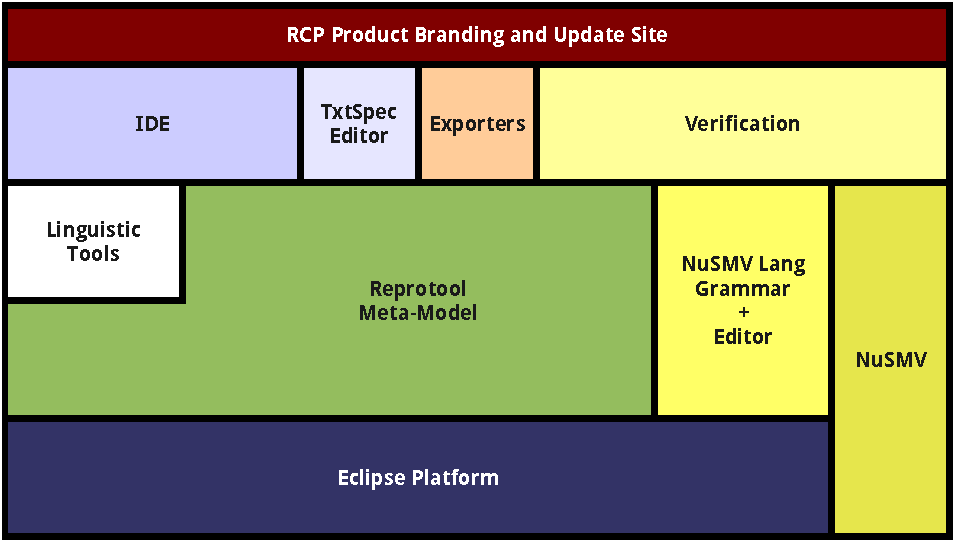
\includegraphics[width=\textwidth]{images/ArchitectureOverview}
  \caption{Reprotool Architecture Overview}
  \label{fig:ArchitectureOverview}
\end{figure}


  \section{Verification of consistency}

A software project specification can be verified for consistency within Reprotool.
This section provides details about the verification process.

The system's behaviour is specified by the set of use-cases contained within the project.
Use-cases and their relations are stored in a memory structure we refer to as a use-case model (Figure~\ref{fig:ReprotoolUCModel}).
The model is based on the EMF framework so that it integrates well within the Eclipse environment.

\begin{figure}[ht]
  \centering
  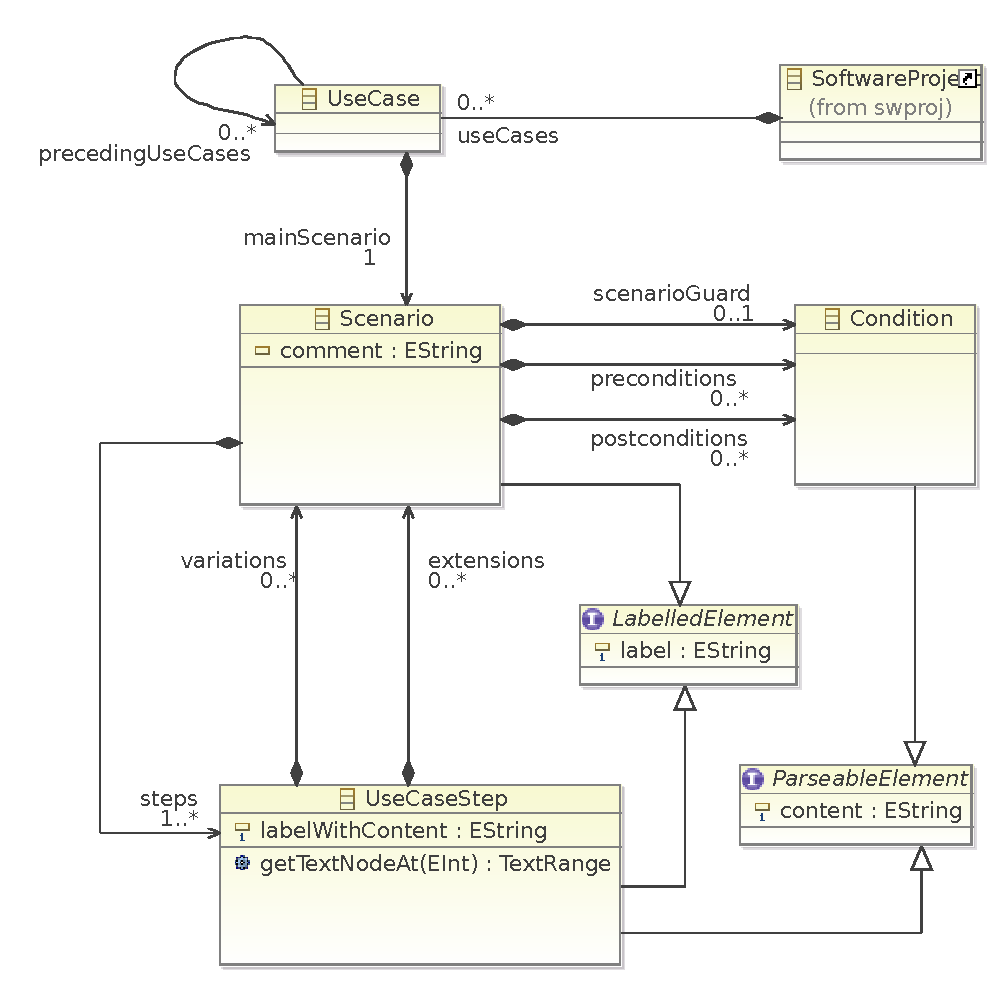
\includegraphics[width=280pt]{images/ReprotoolUCModel}
  \caption{Use-case model}
  \label{fig:ReprotoolUCModel}
\end{figure}

\subsection{Annotations model}

When we refer to verifying the consistency of a system, we actually consider the consistency of temporal properties implied by the annotations used within the project.

Every reprotool project contains a set of temporal constraints imposed upon annotations in the project.
Annotations\footnote{An intuitive example of annotations is the annotation pair \emph{open-close}. For such annotations we could describe constraints like \emph{After open there should always be close}, or \emph{No multi open without close}.} can be attached to individual use-case steps (see \emph{StepAnnotation} element depicted in Figure~\ref{fig:ModelOfAnnotations}).


An annotation attached to a use-case step consists of two parts\footnote{An example of an annotation type we use in Reprotool is \emph{open}.
A suitable \emph{id} for annotation of this type could be \emph{file1}, thus the description of this annotation reads \textcolor{Blue}{\emph{open\_file1}}.}
-- \emph{type} and \emph{id}.

\begin{figure}[ht]
  \centering
  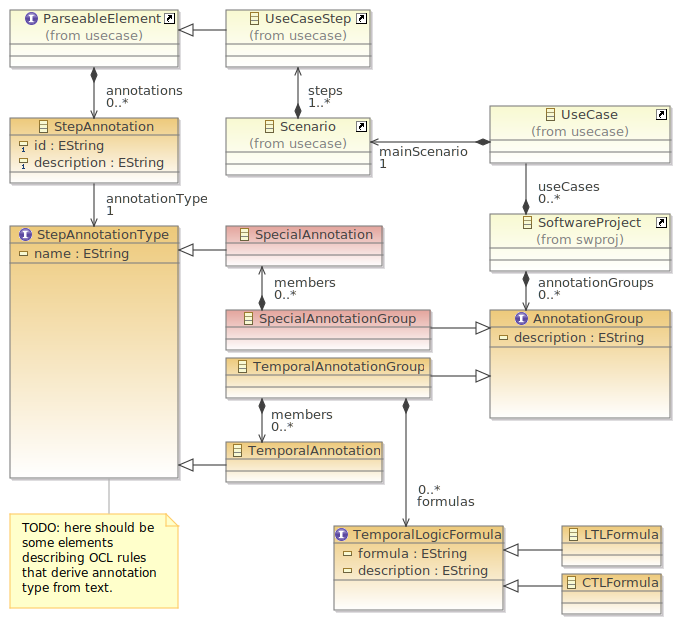
\includegraphics[width=\textwidth]{images/ReprotoolUCAnnotModel}
  \caption{Model of annotations}
  \label{fig:ModelOfAnnotations}
\end{figure}

Every reprotool project specifies a "vocabulary" of annotations (i.e. types of annotations) that users can use to annotate use-case steps. When assigning a \emph{StepAnnotation} to a given step, users would combine \emph{StepAnnotationType} with an arbitrary \emph{id}.

Annotations are organized in groups as depicted in Figure~\ref{fig:ModelOfAnnotations}. Currently, Reprotool supports two kinds of annotations:
\begin{description}

	\item[Temporal annotations] organized in \emph{TemporalAnnotationGroup}s, whose semantics is specified by a set of temporal logic formulae; their format will be described later on.
	
	\item[Special annotations] organized in \emph{SpecialAnnotationGroup}s, whose semantics is hard-coded in Reprotool.
\end{description}

\subsection{Special annotations}

When a \emph{reprotool} user creates a new project from the \emph{Eclipse IDE} new project wizard, a special \emph{trace-on} annotation group is added to the project.
This annotation group contains two special annotations -- \emph{trace} and \emph{on}.
Currently, these are the only special annotations supported by \emph{Reprotool}.
These two special annotations enable the users to select mutually exclusive paths in their use-case scenarios.
This might be used to prune the computation tree the \emph{NuSMV} tool considers when checking the \emph{CTL}/\emph{LTL} specifications.

Let's assume we have a use-case \emph{U} that has the main scenario 7 steps long.
Step 1 and the step 4 have both an extension scenario 3
steps long.
The individual use-case steps are annotated as depicted in the following picture:


\begin{figure}[ht]
  \centering
  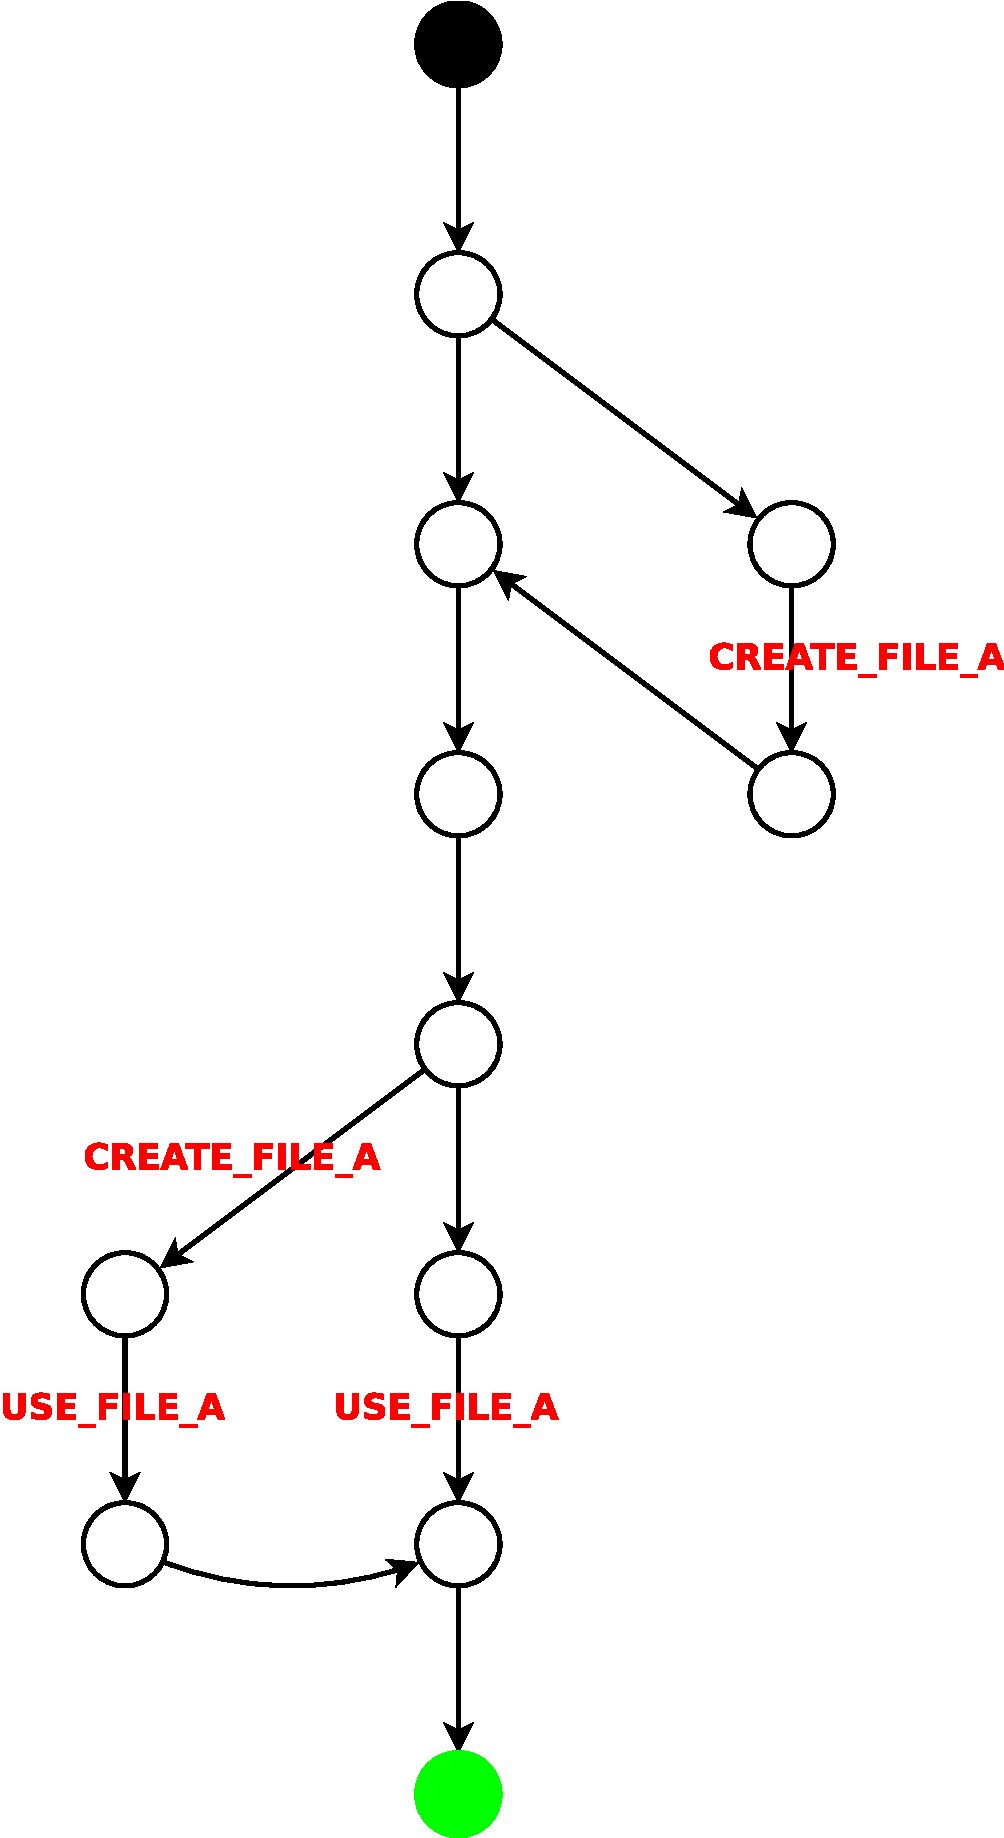
\includegraphics[width=180pt]{images/traceTest_no_trace}
  \caption{Schema of the use-case \emph{U}}
  \label{fig:traceTest_no_trace}
\end{figure}


The use-case \emph{U} contains two annotation types -- \emph{create} and \emph{use}.
One of the constraints imposed on such annotations is a CTL formula:
\begin{verbatim}
CTLSPEC AG( create -> AX(AG(!create)) ) -- Only one 'create'
\end{verbatim}

That means you cannot create a given object more than once.
However, looking at the use-case \emph{U} carefully, it is obvious that there is an execution path containing  the annotation \textcolor{red}{\emph{CREATE\_FILE\_A}} twice.

To solve the problem in the previous example, user needs to specify that if the first extension scenario has been taken, then the second extension scenario of use-case step 4 can not be taken. On the other hand, if the first extension scenario has not been taken,
then the second extension scenario must be taken.
And this is exactly what the \emph{trace} and \emph{on} annotations are for.

\begin{definition}[Semantics of the trace-on annotation pair]
	Let $S$ be a a use-case step.
	Let $on\_x$ be an annotation attached to $S$ (\emph{x} is and arbitrary annotation id).
	Let $T=\{t: S \in t\}$ be a set of all traces going through the step $S$.
	A trace $t \in T$ will be considered for verification only if it contains a step $R'$ annotated with $trace\_x$ before the step $S$.
\end{definition}

Let's clarify it with the help of an example.
In the Figure~\ref{fig:traceTest} you can see the same use-case \emph{U} but with properly added
\emph{trace} and \emph{on} annotations that prevent any conflicts.

\begin{figure}[ht]
  \centering
  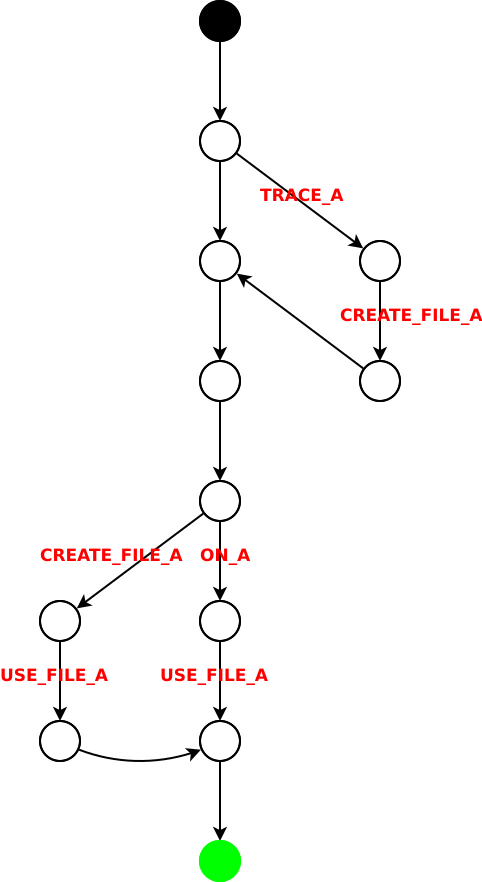
\includegraphics[width=180pt]{images/traceTest}
  \caption{Schema of the use-case \emph{U} with trace/on annotations added}
  \label{fig:traceTest}
\end{figure}

The annotated use-case \emph{U} has now only two execution paths possible. And none of them violates any of the default constraints
imposed on the \emph{create} and \emph{use} annotations. Here you can see the path where the \emph{trace}/\emph{on} branch has been
taken:

\begin{figure}[ht]
  \centering
  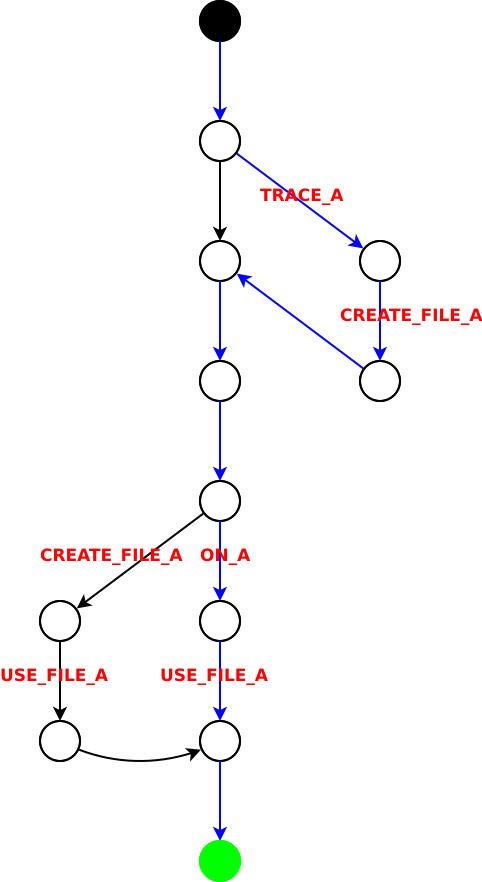
\includegraphics[width=180pt]{images/traceTest_path_taken}
  \caption{\emph{Trace}/\emph{on} branch taken}
  \label{fig:traceTestTaken}
\end{figure}

When the \emph{NuSMV} tool simlates the execution of the state machine corresponding to the annotated use-case \emph{U} and just finished
execution of the 4 step of the use-case main scenario, there would normally by 2 possibilities how to proceed. But because in our
example execution path the \emph{trace\_a} annotaion has been encountered, there is only one possibility - and that is to take the
\emph{on} branch.

\newpage

The situation where the second path has been taken is depicted in the next picture. No other execution paths are considered by the
\emph{NuSMV} tool.

\begin{figure}[ht]
  \centering
  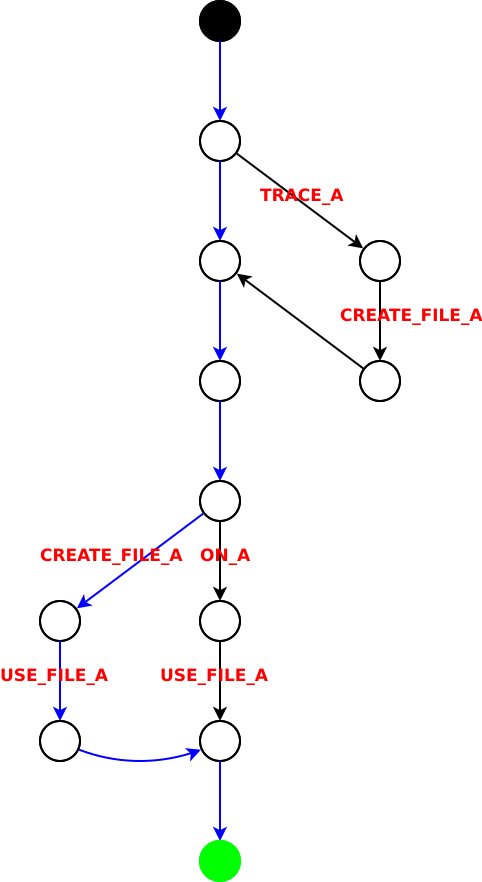
\includegraphics[width=180pt]{images/traceTest_path_not_taken}
  \caption{\emph{Trace}/\emph{on} branch NOT taken}
  \label{fig:traceTestNotTaken}
\end{figure}

\subsection{NuSMV symbolic model checker}

We use NuSMV~\cite{NuSMV-CAV02,NuSMV-frocos02} symbolic model-checker to verify consistency of use-cases with regard to their temporal annotations.
Although NuSMV support BDD-based\footnote{Using binary decision diagrams} and BMC-based\footnote{Bounded model-checking using a SAT solver} model-checking techniques, in our project we use just the BDD-based approach.
NuSMV supports analysis of synchronous and asynchronous systems using Computation Tree Logic (CTL) and Linear Temporal Logic (LTL).
Our framework supports both CTL and LTL, however CTL is preferred because NuSMV would convert LTL formulae into CTL internally (as described in \cite{NuSMV-ltl-fmsd97}).

All use-cases from our UC model have to be converted into NuSMV input language.
We use Xtext\cite{Xtext-website} as a tool for handling DSLs (Domain Specific Languages) which in this case is the NuSMV input language.

NuSMV input language is described using EBNF grammar (inspired by \cite{googlecode-nusmv-tools}) and Xtext generates:
\begin{itemize}
  \item an in-memory representation of the parse tree, sometimes being referred to as an Abstract Syntax Tree (AST),
  \item a text-to-AST parser and
  \item a AST-to-text serializer
\end{itemize}

In order to convert our UC model into NuSMV input language, we use the model-to-model (M2M) approach.
We traverse the UC model and during that traversal we collect the neccesary information to build a new EMF memory structure based on the generaetd NuSMV model.
The generated serializer then produces a valid NuSMV code from the NuSMV model.

\begin{figure}[ht]
  \centering
  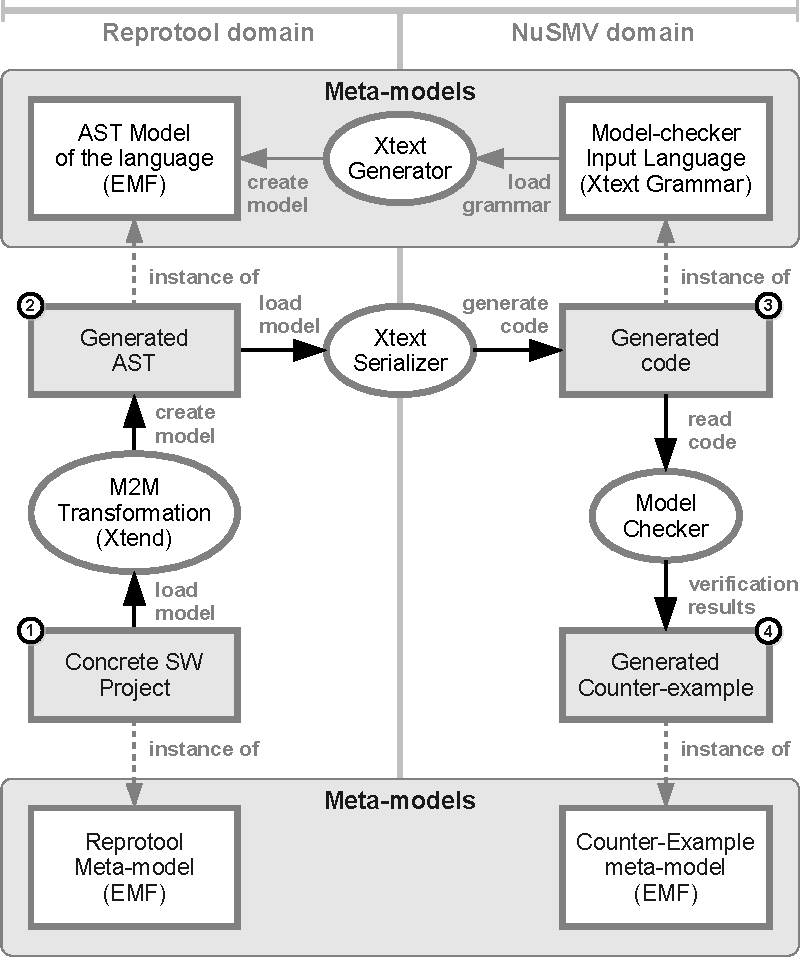
\includegraphics[height=280pt]{images/XtextWorkflow}
  \caption{Transformation of a SW Project into the input language of a model checker}
  \label{fig:XtextWorkflow}
\end{figure}
\pagebreak

\subsection{NuSMV temporal logic formulas}

Temporal annotations of a reprotool project are organised in \emph{TemporalAnnotationGroups}. (See Figure~\ref{fig:ModelOfAnnotations}.)
Every \emph{TemporalAnnotationGroup} contains a set of logically grouped temporal annotations and a set of \emph{temporal logic formulas}
that specify the semantics of the temporal annotations in the group. The NuSMV tool and Reprotool support two types of temporal logic
formulas. And that is:

\begin{enumerate}
 \item CTL (Computation Tree Logic) formulas
 \item LTL (Linear Temporal Logic) formulas
\end{enumerate}

\subsubsection{CTL formulas}
Specify format of CTL formulas

\subsubsection{LTL formulas}
Specify format of LTL formulas

\subsection{Generated NuSMV model}

The NuSMV language model is based on the EMF framework and is generated from the NuSMV language grammar.
This model describes the classes that build up the AST (Abstract Syntax Tree) of the NuSMV language.

Here we present an excerpt from the NuSMV language grammar. You can find the whole grammar in th
\emph{reprotool.fm.nusmv.lang} plugin in the \emph{NuSMVLang.xtext} file.

\begin{lstlisting}[language=XtextGrammar]
grammar reprotool.fm.nusmv.lang.NuSmvLang with org.eclipse.xtext.common.Terminals
generate nuSmvLang "http://d3s.mff.cuni.cz/reprotool/nusmv/lang"
import "http://www.eclipse.org/emf/2002/Ecore" as ecore

Module:
	"MODULE" (MainModule | OtherModule)
	(moduleElement+=ModuleElement)*;
MainModule:
	name='main';

OtherModule:
	name=ID ("(" (params+=FormalParameter) ("," params+=FormalParameter)* ")")?;

ModuleElement hidden(WS, SL_COMMENT):
	  VariableDeclaration
	| IVariableDeclaration
	| FrozenVariableDeclaration
	| DefineDeclaration
	| ConstantsDeclaration
	| AssignConstraint
	| TransConstraint
	| InitConstraint
	| InvarConstraint
	| FairnessConstraint
	| CtlSpecification
	| LtlSpecification
	| InvarSpecification
;
\end{lstlisting}

The Xtext generates an EMF model from the specified grammar. You can have a hierarchical view of the generated model by displaying the
\emph{NuSMVLang.ecore} file in the \emph{reprotool.fm.nusmv.lang} plugin. To better visualise the model, right-click on the \emph{NuSMVLang.ecore} file in
the package explorer of the Eclipse IDE and click the option ``Initialize Ecore Diagram file...''. This will create the \emph{NuSMVLang.ecorediag} file that you can view with the provided Eclipse editor.

% TODO: tento obrazok nesuvisi s textom. Treba ho vyhodit?
\begin{figure}[ht]
  \centering
  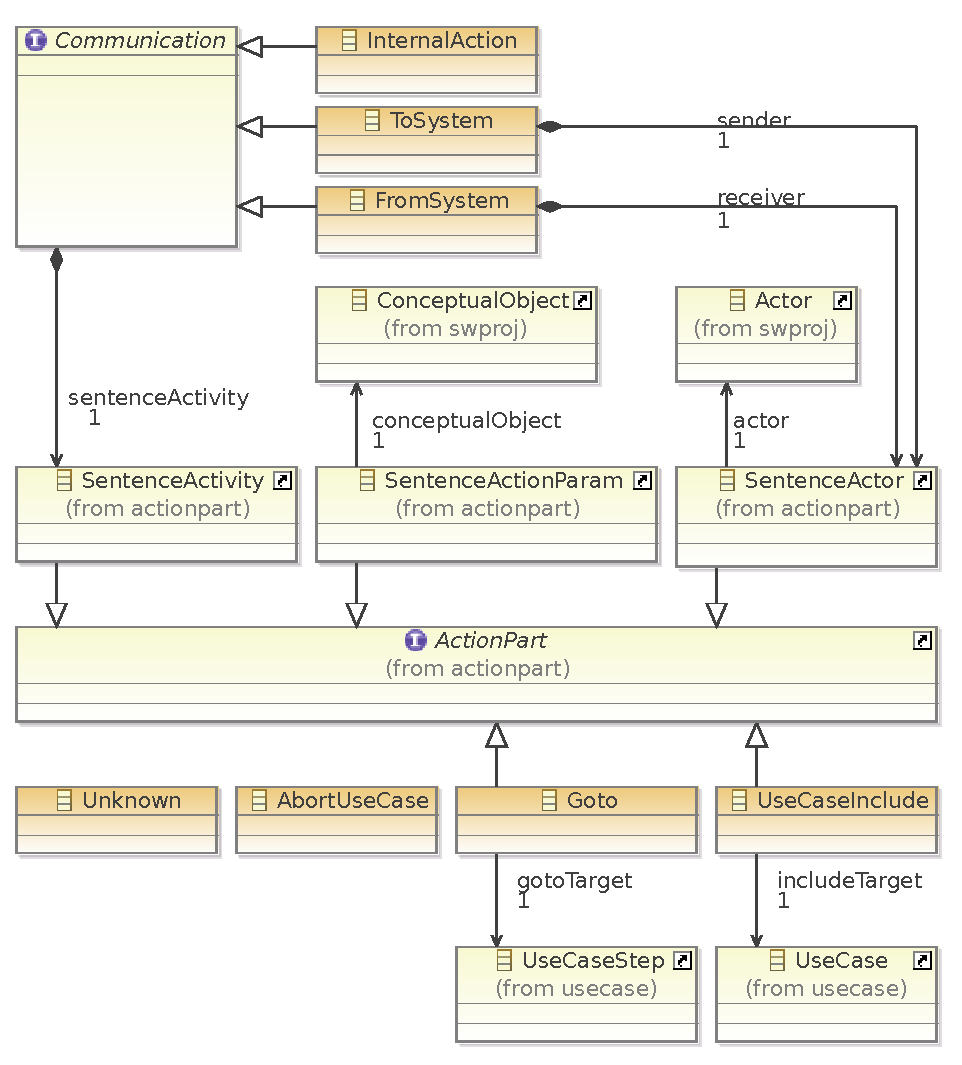
\includegraphics[width=260pt]{images/ReprotoolActionsModel}
  \caption{Model of derived action}
  \label{fig:ReprotoolActionsModel}
\end{figure}

\subsection{Model to model transformation}

Here we present an overview of the transformation of our UC model into the generated NuSMV model. The objective of this process is to take a reprotool project as input and transform it into the generated NuSMV model.

All transformations are implemented using the Xtend~\cite{Xtend-website} language.
Xtend is a statically-typed programming language which is compiled to Java and therefore integrates well and runs on JVM. It brings many concepts simplifying model-to-model and model-to-text transformation. We have leveraged on the following Xtend features: 
\begin{itemize}
	\item Advanced type inference
	\item Extension methods - enhance closed types with new functionality.
	\item Closures - concise syntax for anonymous function literals.
		These features are used for implementing the builder design pattern.
	
		\verb|$(...factory code...)[...initialization code...]|
	
	\item Multiple dispatch a.k.a. polymorphic method invocation.
	\item Operator overloading (e.g. \verb|map += key -> value|)
	\item Property access syntax - shorthands for getter and setter access.
\end{itemize}

This transformation is implemented in the \emph{reprotool.fm.nusmv} plugin in the \emph{reprotool.fm.nusmv.mapping} package.
The transformation itself is quite straight-forward and is defined in an Xtend class \emph{NuSMVProj.xtend}.
For every use-case we create a definition of a non-deterministic state machine.
The state machine's states are directly related to the steps of the related use-case.
The use-cases in the reprotool project can have precedence relations specified. Theses relations are considered in the
transformation process. The use-case state machines are instantiated with a parameter that triggers the execution of the machine.
With this parameter we ensure that the precedence relations are fulfilled. By means of this parameter we also avoid parallel execution
of multiple use-cases.

One part of this model transformation process is to generate NuSMV CTL/LTL formulas which are to be checked by the NuSMV tool. The
skeletons of these formulas are provided by the user in the reprotool project. In this model to model transformation process these
formula skeletons are simply expanded by substituting the annotation patterns with annotations found in the steps of the use-cases
in the reprotool project. A detailed example with explanation is provided in the next section.

\subsection{Example of a reprotool project converted into NuSMV}

In this section we present a simple reprotool project consisting of two use-cases. We show by the means of an example how this project
gets transformed into the NuSMV language format.

The project contains two use-cases. For every use-case U one state machine M is generated. This machine is represented by the states and
transitions between them that are derived directly from the use-case steps of the use-case U. Let's assume our project contains a use
case U1. The use-case U1 has a main scenario that contains five use-case steps. Use-case step 1 is annotated by the annotation \emph{open\_file}
and use-case step 2 is annotated by the annotation \emph{close\_file}. Step 2 has two extension scenarios (One is three steps and the other
one two steps long) and step 4 has one extension scenario two steps long. Step 4 includes another use-case U2 from the project. The
main scenario of use-case U2 contains only single step. You can have a look at the visual representation of the use-case U1 (and also
use-case U2 since it is included in the step 4 of the main scenario of the use-case U1) in the following figure. The initial state is
filled with black colour and the final state is filled with green colour. Steps 1 and 2 are marked with a violet square because these
steps are annotated.

\begin{figure}[h]
  \centering
  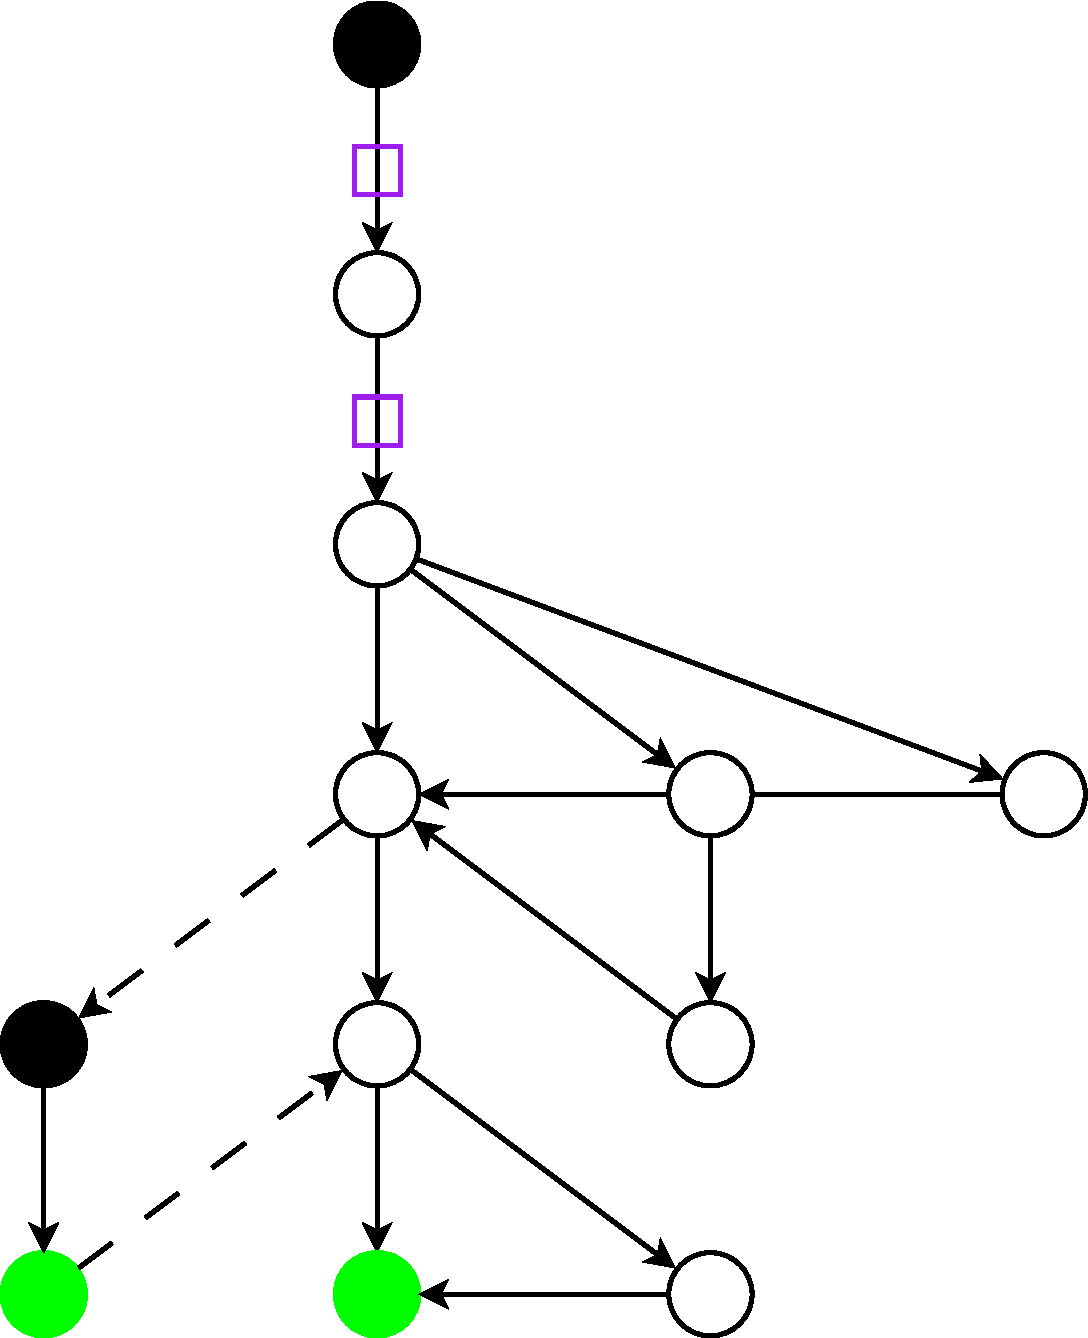
\includegraphics[width=200pt]{images/u1}
  \caption{Visual representation of the use-case U1}
  \label{fig:use-case U1}
\end{figure}

Now we present the state machine M that represents the use-case U1 and is written down using the NuSMV syntax. The state machine is
represented by a single module UC\_U1. This module contains a definition of variable s to which values representing variour machine
states can be assigned. Indeed, the transition to state s1 in the state machine is simulated by assigning the value s1 to the
variable s. The biggest part of the module UC\_U1 specification takes up a case construct that specifies various state transitions
of the machine based on the current state. Becuase use-case U1 includes another use-case U2 (which is represented by the module
UC\_U2), the module UC\_U1 also contains a variable y1 that is an instantiation of the module UC\_U2 included in the module UC\_U1.
\begin{lstlisting}
MODULE UC_U1 ( top , run )
	VAR y1run : boolean ;
	INIT y1run in FALSE
	VAR y1 : UC_U2 ( top , y1run ) ;
	ASSIGN next ( y1run ) := (s=s3__) ;
	VAR s : { s0 , s_ext_3 , s_ext_2 , s2 , s1 , s3__ , s2a2 , s3_ , s2_ , s2b1 ,
		s3a1 , s1_ , s2a1 , s3 , sFin } ;
	INIT s in s0
	ASSIGN next ( s ) := case
		s=s0 & !run : s0;
		s=s0 & run : {s1_};
		s=s3__ & y1.s != sFin : s3__;
		s=s3__ & y1.s  = sFin : s3_;
		s=s_ext_2 : {s3__};
		s=s2 : {s2a1,s2b1,s_ext_2};
		s=s1 : {s2_};
		s=s2a2 : {s_ext_2};
		s=s3_ : s3;
		s=s2_ : s2;
		s=s2b1 : {s_ext_2};
		s=s3a1 : {s_ext_3};
		s=s1_ : s1;
		s=s2a1 : {s2a2};
		s=s3 : {s3a1,s_ext_3};
		s=s_ext_3 : sFin;
		s=sFin : sFin;
	esac ;
\end{lstlisting}

Here we present the machine M2 that represents the included use-case U2.
\begin{lstlisting}
MODULE UC_U2 ( top , run )
	VAR s : { s0 , s1 , sFin } ;
	INIT s in s0
	ASSIGN next ( s ) := case
		s=s0 & !run : s0;
		s=s0 & run : {s1};
		s=s1 : sFin;
		s=sFin : sFin;
	esac ;
\end{lstlisting}

As we have already mentioned when describing use-case U1, the first two steps of its main scenario are annotated. (This is denoted
by a small violet square in the graphical representation of the use-case U1). Every such an annotation generates an annotation variable
definition in the NuSMV model. The variable name encodes the annotation type (for example open) and the annotation id (for example
file1). The variable is of boolean type and is initialized with the logical value of zero. The variable value is set to logical one
if and only if the state variable s of the respective state machine module denotes that the machine is in the annotated state.

Let's clarify this a bit more with the example of our project. There we have use-case step one of the use-case U1 annotated with the
open annotation (annotation id is file1) and step two annotated with the close annotation (annotation id is file1). These two use-case
step annotations in the use-case U1 of our project yield the following annotation variable definitions:

\begin{lstlisting}
VAR open_file1 : boolean ;
INIT open_file1 in FALSE
ASSIGN next ( open_file1 ) := FALSE
	| xU1.s in {s1_} ;
VAR close_file1 : boolean ;
INIT close_file1 in FALSE
ASSIGN next ( close_file1 ) := FALSE
	| xU1.s in {s2_} ;
\end{lstlisting}

Now we will describe the variable named \emph{p} which has the function of a steering wheel of whole simulation performed by the \emph{NuSMV} tool
when looking for possible violations of our system. This variable is of type enum and can assume the value \emph{none}, or other n values that
map directly to the n use-cases present in our project. The \emph{p} variable is initialised with the \emph{none} value. When the \emph{NuSMV} tool performs
steps in our system which are basicly transitions in the state machines of our use-cases, the value of the \emph{p} variable alternates between
the \emph{none} value and any other value from the set of possible values. Thus, the \emph{p} variable definition looks like this:
\begin{lstlisting}
VAR p : { none , pU1 , pU2} ;
INIT p in none
ASSIGN next ( p ) := case
	p=none : {pU1, pU2};
	TRUE : none;
esac ;
\end{lstlisting}

The \emph{p} variable helps us to decide which state machine could be executed in the next steps. We also generate definition for the
boolean variable \emph{idle} that tells us if any of the use-case state machines is currently being executed. The \emph{idle} variable is defined
by the means of a set of boolean variables from which every variable tells us if the machine to which it maps is currently
being executed. This is how it looks in the \emph{NuSMV} syntax:
\begin{lstlisting}
VAR idle : boolean ;
INIT idle in TRUE
ASSIGN next ( idle ) := case
	xU1run | xU2run : FALSE;
	TRUE : TRUE;
esac ;
\end{lstlisting}

Next we need to define for every use-case \emph{UN} a boolean variable \emph{xUNrun} that triggers the execution of the respective state machine
and at the same time serves as an indicator if the respective state machine N is currently running. This boolean variable is
initialised with logical zero. It is assigned the logical one only if all other machines are idle and the p variable points to the
machine N. For every use-case UN we also need to define a variable \emph{xUN} that is the actual instantiation of the state machine N.
Of course this variable is of type \emph{UC\_UN}. This is how the definitions of the variables \emph{xUN} and \emph{xUNrun} look in practice:
\begin{lstlisting}
VAR xU1 : UC_U1 ( self , xU1run ) ;
VAR xU1run : boolean ;
INIT xU1run in FALSE
ASSIGN next ( xU1run ) := case
	p=pU1 & idle & xU1.s = s0 : TRUE;
	TRUE : xU1run & xU1.s != sFin;
esac ;
\end{lstlisting}

Now we are going to describe how the \emph{CTL} and \emph{LTL} specifications are generated. When a new empty reprotool project is generated in the
\emph{Eclipse IDE}, it already contains a set of predefined \emph{CTL} formulas along with a quick description of each formula. Here is a subset of
these predefined formulas that is relevant to the \emph{open}/\emph{close} annotations:

\begin{description}
 \item [$AG(open \rightarrow AF(close))$] After 'open' there should always be 'close'
 \item [$AG(open \rightarrow AX(A\lbrack!open \cup close\rbrack))$] No multi-open without close
 \item [$AG(close \rightarrow AX(A\lbrack!close \cup open \mid !AF(close) \rbrack))$] No multi-close without open
 \item [$A\lbrack !close \cup open \mid !AF(close)\rbrack$] First 'open' then 'close'
\end{description}

We can see that these logical formulas specify properties for the open and close annotations. We also know that in the use-case \emph{U1} we
use annotation \emph{open\_file1} and \emph{close\_file1}. Now we simply expand the predefined \emph{CTL} and \emph{LTL} formulas. This is what we get in our
example:
\begin{lstlisting}
CTLSPEC AG(open_file1 -> AF(close_file1))
CTLSPEC AG(open_file1 -> AX(A[!open_file1 U close_file1]))
CTLSPEC AG(close_file1 -> AX(A[!close_file1 U open_file1 | !AF(close_file1) ]))
CTLSPEC A[!close_file1 U open_file1 | !AF(close_file1)]
\end{lstlisting}

And this is what the \emph{NuSMV} file looks like:
\begin{lstlisting}
MODULE main
	CTLSPEC AG(open_file1 -> AF(close_file1))
	CTLSPEC AG(open_file1 -> AX(A[!open_file1 U close_file1]))
	CTLSPEC AG(close_file1 -> AX(A[!close_file1 U open_file1 | !AF(close_file1) ]))
	CTLSPEC A[!close_file1 U open_file1 | !AF(close_file1)]

	FAIRNESS p=pU1
	FAIRNESS p=pU2
	FAIRNESS p=pU3

	VAR p : { none , pU1 , pU2} ;
	INIT p in none
	ASSIGN next ( p ) := case
		p=none : {pU1, pU2};
		TRUE : none;
	esac ;

 	VAR idle : boolean ;
	INIT idle in TRUE
	ASSIGN next ( idle ) := case
		xU1run | xU2run : FALSE;
		TRUE : TRUE;
	esac ;

 	VAR xU1 : UC_U1 ( self , xU1run ) ;
	VAR xU1run : boolean ;
	INIT xU1run in FALSE
	ASSIGN next ( xU1run ) := case
		p=pU1 & idle & xU1.s = s0 : TRUE;
		TRUE : xU1run & xU1.s != sFin;
	esac ;

	VAR xU2 : UC_U2 ( self , xU2run ) ;
	VAR xU2run : boolean ;
	INIT xU2run in FALSE
	ASSIGN next ( xU2run ) := case
		p=pU2 & idle & xU2.s = s0 : TRUE;
		TRUE : xU2run & xU2.s != sFin;
	esac ;

 	VAR open_file1 : boolean ;
	INIT open_file1 in FALSE
	ASSIGN next ( open_file1 ) := FALSE
		| xU1.s in {s1_}
	;

	VAR close_file1 : boolean ;
	INIT close_file1 in FALSE
	ASSIGN next ( close_file1 ) := FALSE
		| xU1.s in {s2_}
	;

MODULE UC_U1 ( top , run )
	VAR y1run : boolean ;
	INIT y1run in FALSE
	VAR y1 : UC_U2 ( top , y1run ) ;
	ASSIGN next ( y1run ) := (s=s3__) ;
	VAR s : { s0 , s_ext_3 , s_ext_2 , s2 , s1 , s3__ , s2a2 , s3_ , s2_ , s2b1 ,
			s3a1 , s1_ , s2a1 , s3 , sFin } ;
	INIT s in s0
	ASSIGN next ( s ) := case
		s=s0 & !run : s0;
		s=s0 & run : {s1_};
		s=s3__ & y1.s != sFin : s3__;
		s=s3__ & y1.s  = sFin : s3_;
		s=s_ext_2 : {s3__};
		s=s2 : {s2a1,s2b1,s_ext_2};
		s=s1 : {s2_};
		s=s2a2 : {s_ext_2};
		s=s3_ : s3;
		s=s2_ : s2;
		s=s2b1 : {s_ext_2};
		s=s3a1 : {s_ext_3};
		s=s1_ : s1;
		s=s2a1 : {s2a2};
		s=s3 : {s3a1,s_ext_3};
		s=s_ext_3 : sFin;
		s=sFin : sFin;
	esac ;

MODULE UC_U2 ( top , run )
	VAR s : { s0 , s1 , sFin } ;
	INIT s in s0
	ASSIGN next ( s ) := case
		s=s0 & !run : s0;
		s=s0 & run : {s1};
		s=s1 : sFin;
		s=sFin : sFin;
	esac ;
\end{lstlisting}

  \section{UML Export}

The \emph{reprotool.uml.export} plugin is responsible for exporting a \emph{reprotool} project into UML. A \emph{reprotool} user has
a possibility to create either a \emph{UML class diagram} or a \emph{UML use case diagram}. The UML model we use in \emph{reprotool}
comes from the \emph{org.eclipse.uml2.uml} eclipse plugin. This model is based on the EMF framework.

\subsection{UML class diagram}
The \emph{UML class diagram} contains class entities for every project actor and one class entity representing the \emph{system}.
The actors in the diagram are provided with activities that they perform.

\begin{figure}[ht]
  \centering
  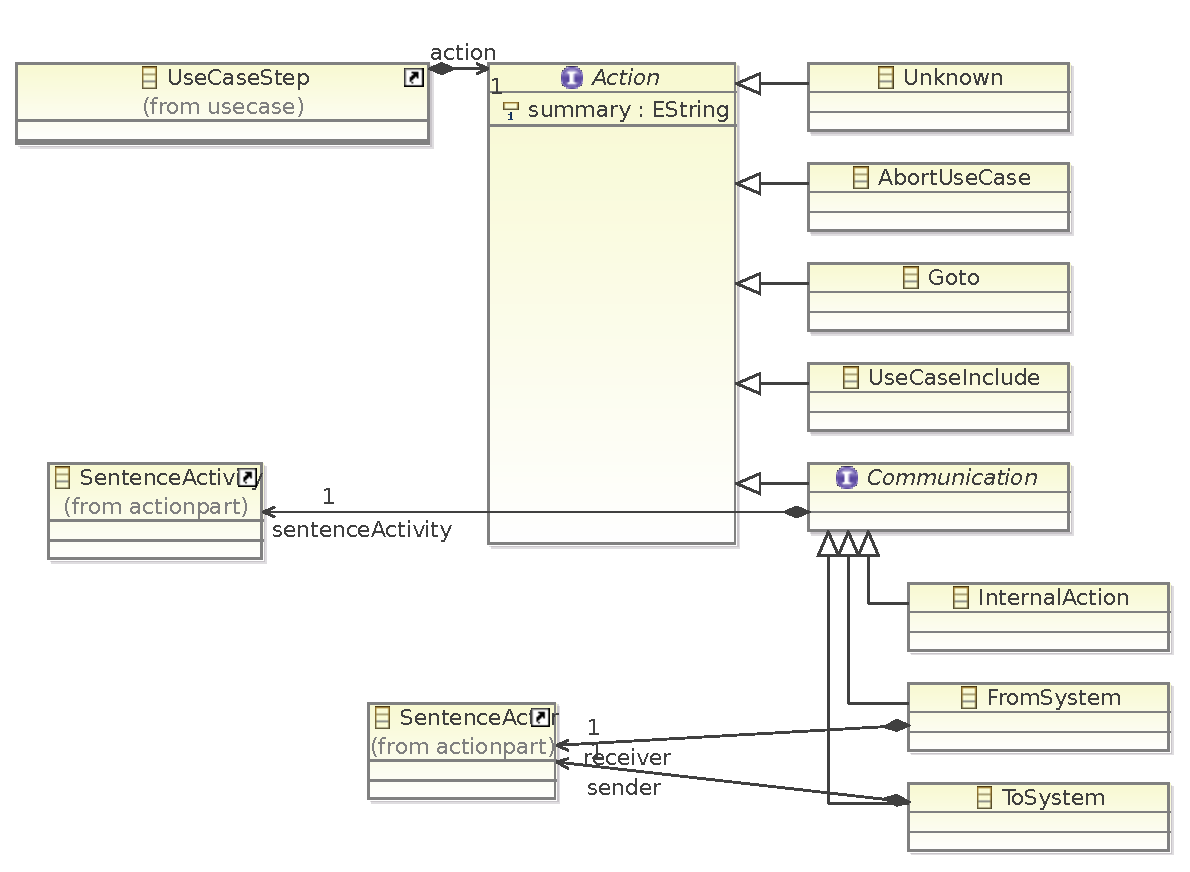
\includegraphics[width=\textwidth]{images/ReprotoolActionsModelSimple}
  \caption{Model of use-case step actions}
  \label{fig:ReprotoolActionsModel}
\end{figure}

Every use-case step can specify an activity for some
actor. This is achieved by assigning an \emph{action} of the type \emph{Communication} to the use-case step. The \emph{Communication}
actions can be either \emph{InternalAction}, \emph{FromSystem}, or \emph{ToSystem}. If the action is of type \emph{InternalAction},
or \emph{ToSystem}, the associated activity is performed on the actor representing the \emph{system}. Otherwise, if the action is of
type \emph{FromSystem}, the \emph{receiver} of the action determins the actor associated with the activity.

The UML class diagram model is generated in the \emph{UMLGen.xtend} class in the \emph{reprotool.uml.export.mapping} package of the
\emph{reprotool.uml.export} plugin. This whole process is simply a transformation of our use-case model into the UML class diagram
model. We utilised \emph{XTend} for this process to take advantage of some of its functional programming language features.

\subsection{UML use-case diagram}
The \emph{UML use-case diagram} contains actor entities for every project actor and use-case entities for every project use-case.
For every project use-case \emph{U} that has its \emph{primary actor} set, the diagram also contains a link between the use-case \emph{U}
and its primary actor. The diagram also depicts the \emph{include} relation between project use-cases. An \emph{include} relation between
two use-cases \emph{U1} and \emph{U2} will appear in the diagram, if there exists at least one execution path in use-case \emph{U1}
that contains a use-case step that includes use-case \emph{U2}.

The UML use-case diagram model is generated in the \emph{UMLUseCaseModelGenerator.xtend} class in the \emph{reprotool.uml.export.mapping} package of the
\emph{reprotool.uml.export} plugin. The whole process is a simple two-phase model transformation process. In the first phase, the
information about project actors and their associated use-cases is collected. In the second phase, the use-case include relations are
searched.


  \section{Label Transition System}

\emph{Reprotool} users work by editing use-cases using our use-case editor. The in-memory representation of actual use-cases are java
objects that are modelled according to our use-case model. (See a simplified view of the model in Figure~\ref{fig:ReprotoolUCModel})
While this model is very useful, it is also quite complex. In some cases we find it helpful to take just a simplified view of a
use-case and consider it a state machine. Every use-case has a main scenario that has a first use-case step, a last step (They could,
however, be the same step) and possibly some other steps. That is analogical to a state machine that has a initial state, an accepting
state and possibly some other states. The model that describes the building blocks of this state machine is based on the EMF and is
called \emph{Label Transition System}.

We use the \emph{LTS} in \emph{Reprotool} when we create NuSMV state machines from use-cases that are used during the NuSMV
verification. We also take advantage of the \emph{LTS} when we create a graphical view of a use-case in the outline view of the
use-case editor. The \emph{LTS} model is depicted in the following figure.

\begin{figure}[ht]
  \centering
  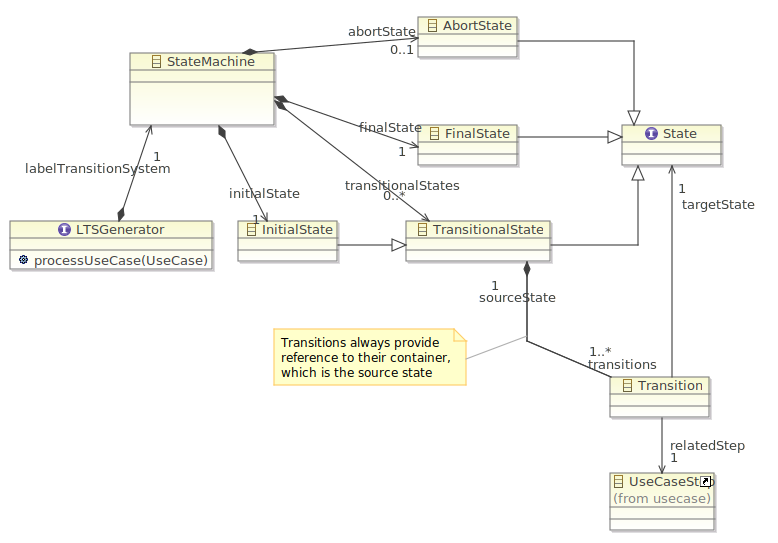
\includegraphics[width=450pt]{images/lts}
  \caption{\emph{LTS} model}
  \label{fig:ReprotoolLTSModel}
\end{figure}

Now, we will describe in more detail the way how the \emph{LTS} state machine is constructed from some use-case \emph{U}.

\subsection{Variation scenario}
If a use-case step \emph{s} has a variation scenario specified, that means either the step \emph{s} is taken, or its variation scenario is
taken. Not both of them. After the variation scenario is performed, the execution continues after the step \emph{s}. (But if the
last step of the variation scenario has a \emph{goto} action specified, the execution continues at step that is specified as
\emph{goto} target.)

This is depicted in the next figure that shows a simple use-case \emph{U} and the use-case \emph{U\'} with a variation
scenario added to the second step (the red one). The variation scenario is two steps long.
Notice the placement of the variation branch in the picture and also notice that an additional transition \emph{t} (the blue one)
has been added to the \emph{LTS} diagram that determines where the execution continues after the variation scenario. This transition
\emph{t} is not directly related to any of the use-case steps of the use-case \emph{U}. All other \emph{LTS} transitions have a
corresponding use-case step in the use-case \emph{U} or in the variation scenario.

\begin{figure}[ht]
  \centering
  
\includegraphics[width=200pt]{images/variation}
  \caption{Use-case \emph{U} and use-case \emph{U\'} with a variation scenario added}
  \label{fig:VariationScenario}
\end{figure}

\subsection{Extension scenario}
If a use-case step \emph{s} has an extension scenario specified, that means after the step \emph{s} is taken, the extension scenario
might be taken. After the extension scenario is performed, the execution continues after the step \emph{s}. (But if the
last step of the extension scenario has a \emph{goto} action specified, the execution continues at step that is specified as
\emph{goto} target.)

This is shown in the next figure that shows a simple use-case \emph{U} and the use-case \emph{U\'} with an extension scenario added
to the first step (the red one). The extension scenario is two steps long.
Notice the placement of the extension branch in the picture and also notice that two additional transitions (the blue ones) have been
added to the \emph{LTS} diagram. One blue transition has been added at the end of the extension scenario and it determines where
the execution continues after the extension scenario is performed. The second blue transition has been added between the red and the
violet use case step - these are consecutive in the original use-case \emph{U}. This second blue transition is taken if the extension
scenario is not taken. Again, the blue transitions do not have a corresponding use-case step. All other transition have one - either
in the original use-case \emph{U} or in the extension scenario.

\begin{figure}[ht]
  \centering
  
\includegraphics[width=200pt]{images/extension}
  \caption{Use-case \emph{U} and use-case \emph{U\'} with an extension scenario added}
  \label{fig:ExtensionScenario}
\end{figure}

\subsection{LTS visualisation}

We use \emph{Zest: The Eclipse Visualization Toolkit} for displaying the LTS diagram in the outline view of the use-case editor and
in the outline view of the \emph{CounterExample} editor. The \emph{CounterExample} editor is the eclipse editor plugin that
gets fired up when a \emph{Reprotool} user double-clicks the counter-example file generated by the NuSMV tool after the verification
process. The \emph{Zest} toolkit is used for displaying graph-like structures in eclipse plugins. The entire library is built on top of SWT/Draw2D so that
it integrates well within eclipse.
  \section{Linguistic tools}

One of the main parts of Reprotool project is an automated analysis of the use case steps. This functionality saves user's work with tedious manual annotation - all the user has to do is to push a button. However, if user is not satisfied with results he can always manually tweak the analyzed use case step. This chapter describes implementation of linguistics analysis in Reprotool project and its linguistics background.

\subsection{Introduction}
Process of linguistic analysis gets natural language sentences as an input and returns analyzed usecases as is shown at figure \ref{fig:LinguisticsAnalyseSmall}. Whole process is divided into two parts: process of parsing and core analysis. Parsing contains main linguistic operations which are tokenization, tagging, parsing and lemmatization. Core work of parsing process is done by popular external linguistic analysis tools described in section \ref{sec:externaltools}. Core analysis converts parsed sentence trees with annotations into our usecases model. This process is described in more detail in section \ref{sec:analysis}. 

It is recommended to see section \ref{sec:analyzer}, where is also located our linguistic model at figure \ref{fig:ReprotoolLingModel}.

\begin{itemize}
\item {\bf Text preparation} Cleaning up input text and tokenization
\item {\bf Dependency trees} POS tagging and parsing
\item {\bf Constituents} determining important text ranges
\item {\bf Action type} final output result of analysis
\end{itemize}

Each implementation of any analyse brings problem of measuring success. We have put together a dataset of nearly three hundred sentences. These sentences contain the most common use cases operations. All these sentences were manually annotated and analyzed. In section \ref{sec:benchmark} is described our benchmark solution with actual results.

\begin{figure}[ht]
  \centering
  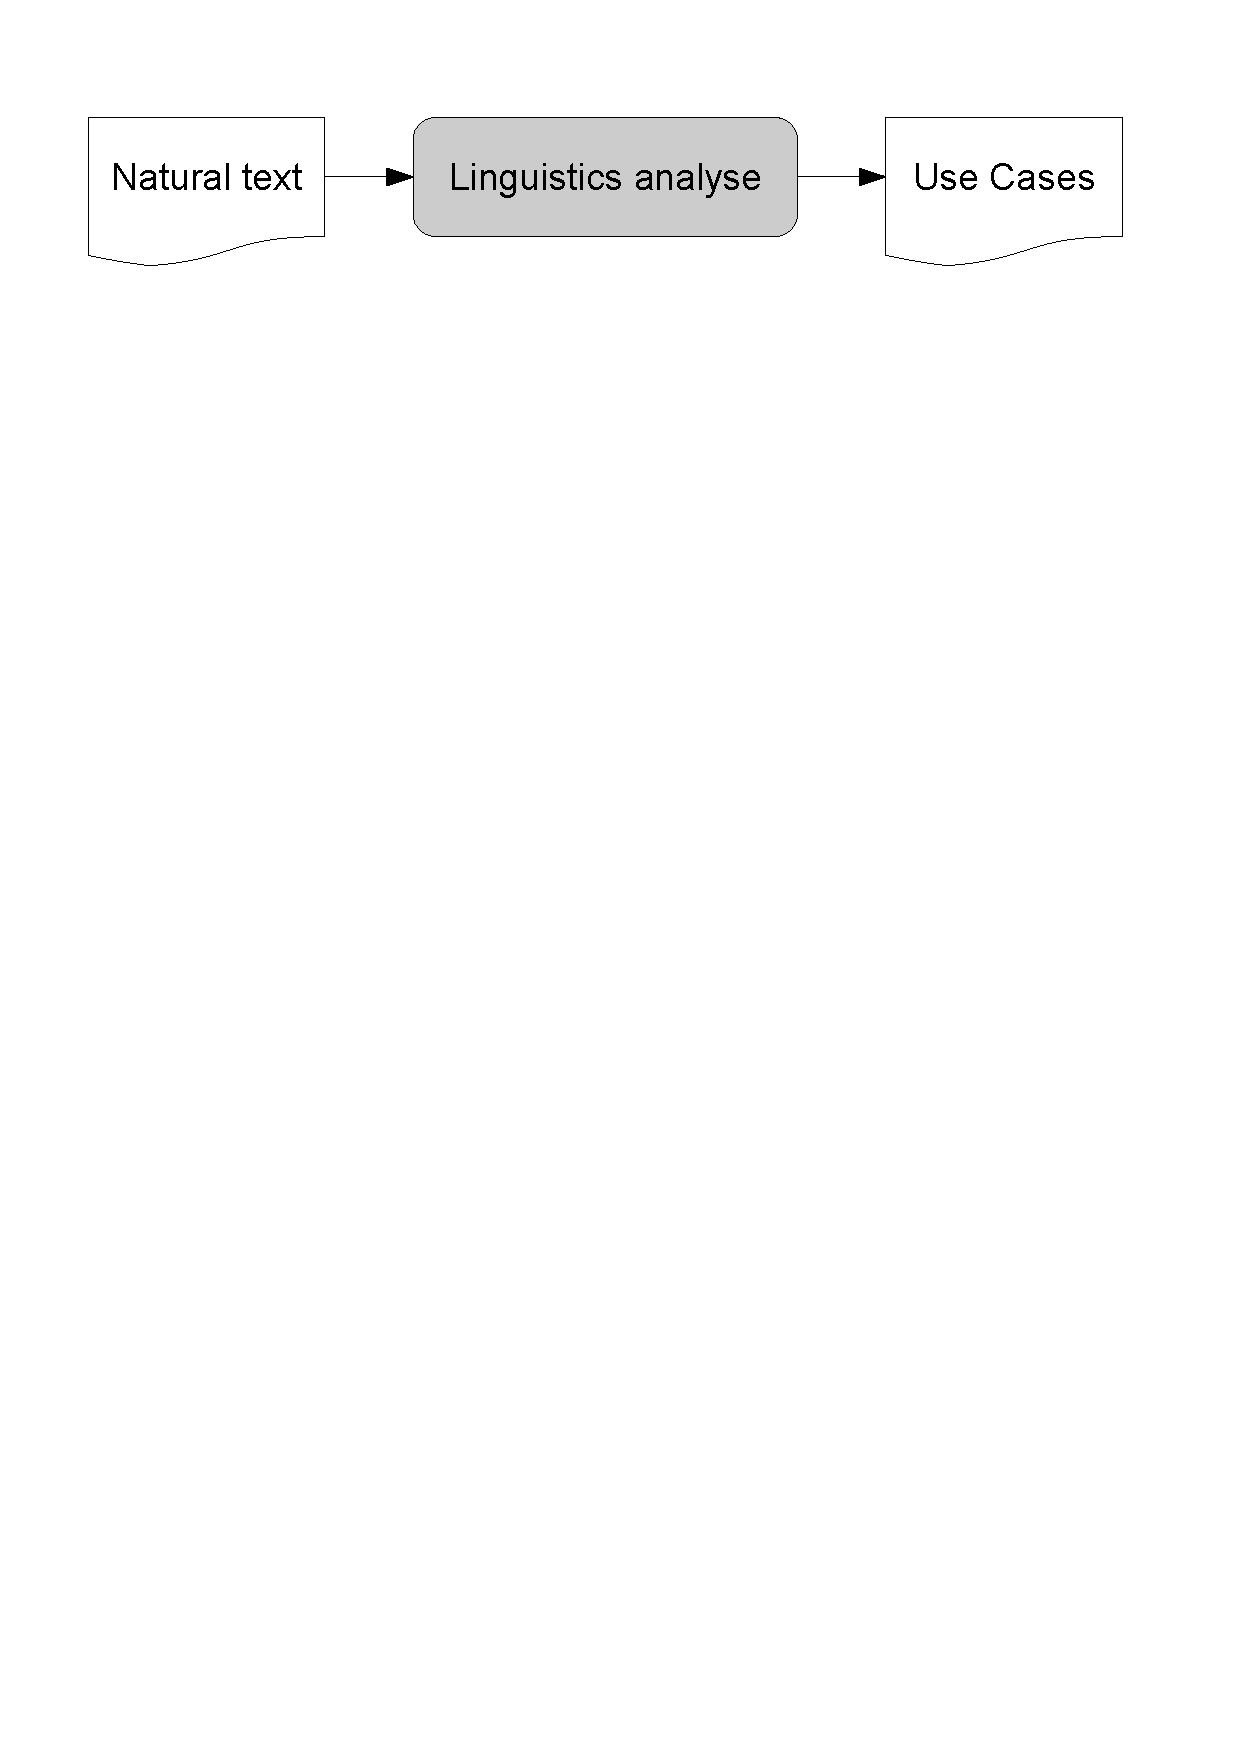
\includegraphics[height=30pt]{images/LinguisticsAnalyseSmall}
  \caption{Process of sentence analysis}
  \label{fig:LinguisticsAnalyseSmall}
\end{figure}

Following pages contain description of the used linguistics tools. All tools use Penn TreeBank tags notation. We use this notation in our model and our tools as well.

\subsection{External tools}
\label{sec:externaltools}
As described in previous sections whole process of linguistics analysis is not a trivial task. We chose commonly used external tools for some parts of analysis and bundled them as Eclipse plugins.

These parts were \emph{part-of-speech tagging}, \emph{sentence parsing} and \emph{obtaining lemma forms} for words. Main reasons for our selection were widespread usage and credibility of the tools, at least partial compatibility of output and input formats and Java implementation. 

We demanded Java implementation, because runtime control of programs written in different languages is inoperative and bring problems in portability of the project. The selected tools don't provide access to analysed entities in form of Java objects, but we are able to control their correct running.

Needed models for all tools are build and packed with bundles corresponding to these tools. These bundles are \verb|reprotool.tools.anna|,  \verb|reprotool.tools.dbparser| and \verb|reprotool.tools.mxpost|.


Selected tools are:
 
\begin{itemize}
\item {\bf MXPOST tagger} - \href{http://www.inf.ed.ac.uk/resources/nlp/local_doc/MXPOST.html}{Java implementation of well known Maximum Entropy Part-Of-Speech Tagger}
\item {\bf Dan Bikel's Multilingual Statistical Parsing Engine } - Java implementation coming from \href{http://www.cis.upenn.edu/~dbikel/software.html#stat-parser}{Dan Bikel’s Home Page}
\item {\bf Mate-tools lemmatizer} - part of bigger project called \href{http://code.google.com/p/mate-tools/}{Tools for Natural Language Analysis}
\end{itemize}

Larger list of tools could be found at project site. There are also links to similar pages concerned with the same theme. 
          
\subsubsection{MXPOST tagger} 
MXPOST tagger was written in Java implementation at University of Edinburg by NLP group and is maintained as part of theirs NLP tools.
        
Main part of this tagger is based on original parser written by Adwait Ratnaparkhi. Detailed description of this original parser is described in article \cite{Linguistics-ratnaparkhi96} and in his PhD thesis \cite{Linguistics-ratnaparkhi98}. 

Input data, natural language sentences, have to be tokenized according to the Penn Treebank conventions. Tagger needs for the run its model consisting of tagged data. Input data are then tagged with use of maximum entropy probability distribution. So the tagger has to find sentence with similar structure in the trained data.
  
\subsubsection{Dan Bikel's Multilingual Statistical Parsing Engine}   

Statistical parsing engine does two main tasks. First is creating and training of the model and second is core parsing. For these purposes we had to obtain large data model with parsed sentences. 

During the parsing, parser is trying to find the most similar sentence in trained model. As a trained data, we use a part of \emph{Penn Treebank, Wall Street Journal collection}.

\subsubsection{Mate-tools lemmatizer}          
          
This lemmatizer is working in a similar way like previous parser. It also needs similar data models, because it cannot use just list of lemmas and their word forms. It also needs to obtain POS information for correct work.

This tool uses one word per line 2009 CoNLL input format, so we had to divide our sentences to adapt them to this format.

\subsection{Linguistic analysis}
\label{sec:analysis}
Linguistics analysis covers multiple different actions executed by various tools. Connection of these tool is described at figure \ref{fig:LinguisticsAnalyse}. In this section are described only pure linguistic tools. Core structure of our action type determining analyzer is described in section \ref{sec:analyzer}.

All tools have at least our wrapper. This wrapper tries to keep selected tool running if possible. This speeds up analysis approximately ten times.

As you can see, this pipeline obtains structure similar to dependency tree for each sentence. We are storing for each sentence this dependency tree. For each word in sentence we also store POS tag and lemma form.

\begin{figure}[ht]
  \centering
  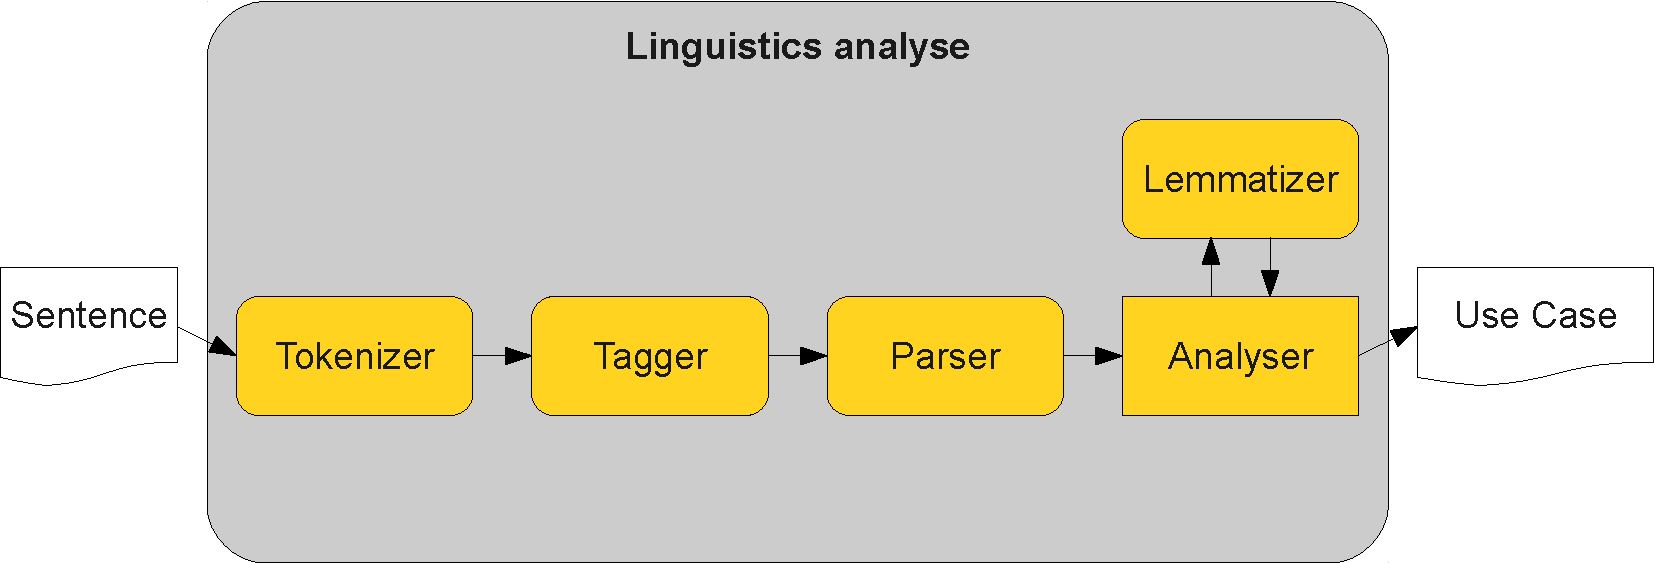
\includegraphics[width=400pt]{images/LinguisticsAnalyse}
  \caption{Process of sentence analysis}
  \label{fig:LinguisticsAnalyse}
\end{figure}

As we can see, the biggest problem is data conversion between two following tools. These important actions are described by input and output data of each task.

\subsubsection{Tokenization}
First part of natural language processing is provided by our own tokenizer. Tokenizer splits sentence into set of separated strings called tokens. These tokens are base units for natural language processing. Each token usually represents one word, a number or punctuation. Invalid tokens are striped by following tools, but these tools are not stripping parts of the tokens.

\begin{table}[ht]   % or b
\begin{center}
  \begin{tabular}{| r | l |}
\hline
Input 	&	Natural language sentence \\ \hline
Output &	Array of tokens (eg. words, numbers) \\ 
\hline
  \end{tabular}
  \caption{Tokenizer data formats}
  \label{tab.tokenization}
\end{center}
\end{table} 

    


\subsubsection{Tagging}
Tagging adds information for each word. Usually determines part of the speech, but it can also obtain more linguistic categories. We use external POS tagger and our analysis uses only POS information.

\begin{table}[ht]   % or b
\begin{center}
  \begin{tabular}{| r | l |}
\hline
Input 	& Array of tokens \\ \hline
Output 	& Array of POS tagged tokens (eg. adjectives, verbs) \\ 
\hline
  \end{tabular}
  \caption{Tagger data formats}
  \label{tab.tagging}
\end{center}
\end{table} 


\subsubsection{Parsing}
Main task of parser is creation of the dependency tree for each sentence. Parser determines all sentence parts and their types. It also sets their interdependences. For better explanation, example of parsed tree could be found at figure \ref{fig:ParsedTree}.

Our project uses external parser wrapped into Eclipse plugin. 


\begin{table}[ht]   % or b
\begin{center}
  \begin{tabular}{| r | l |}
\hline
Input 	& Array of POS tagged tokens \\ \hline
Output 	& Parse trees of each sentence \\ 
\hline
  \end{tabular}
  \caption{Parser data formats}
  \label{tab.parsing}
\end{center}
\end{table} 



\subsubsection{Lemmatization}
Lemmatization basically means finding lemma forms for all words in a sentence. As stated, we are using external tool for this purpose wrapped in Eclipse plugin.

\begin{table}[ht]   % or b
\begin{center}
  \begin{tabular}{| r | l |}
\hline
Input 	& Parse trees of each sentence \\ \hline
Output 	& Lemma for each word \\ 
\hline
  \end{tabular}
  \caption{Lemmatizer data formats}
  \label{tab.lemmatizer}
\end{center}
\end{table} 


\begin{figure}[ht]
  \centering
  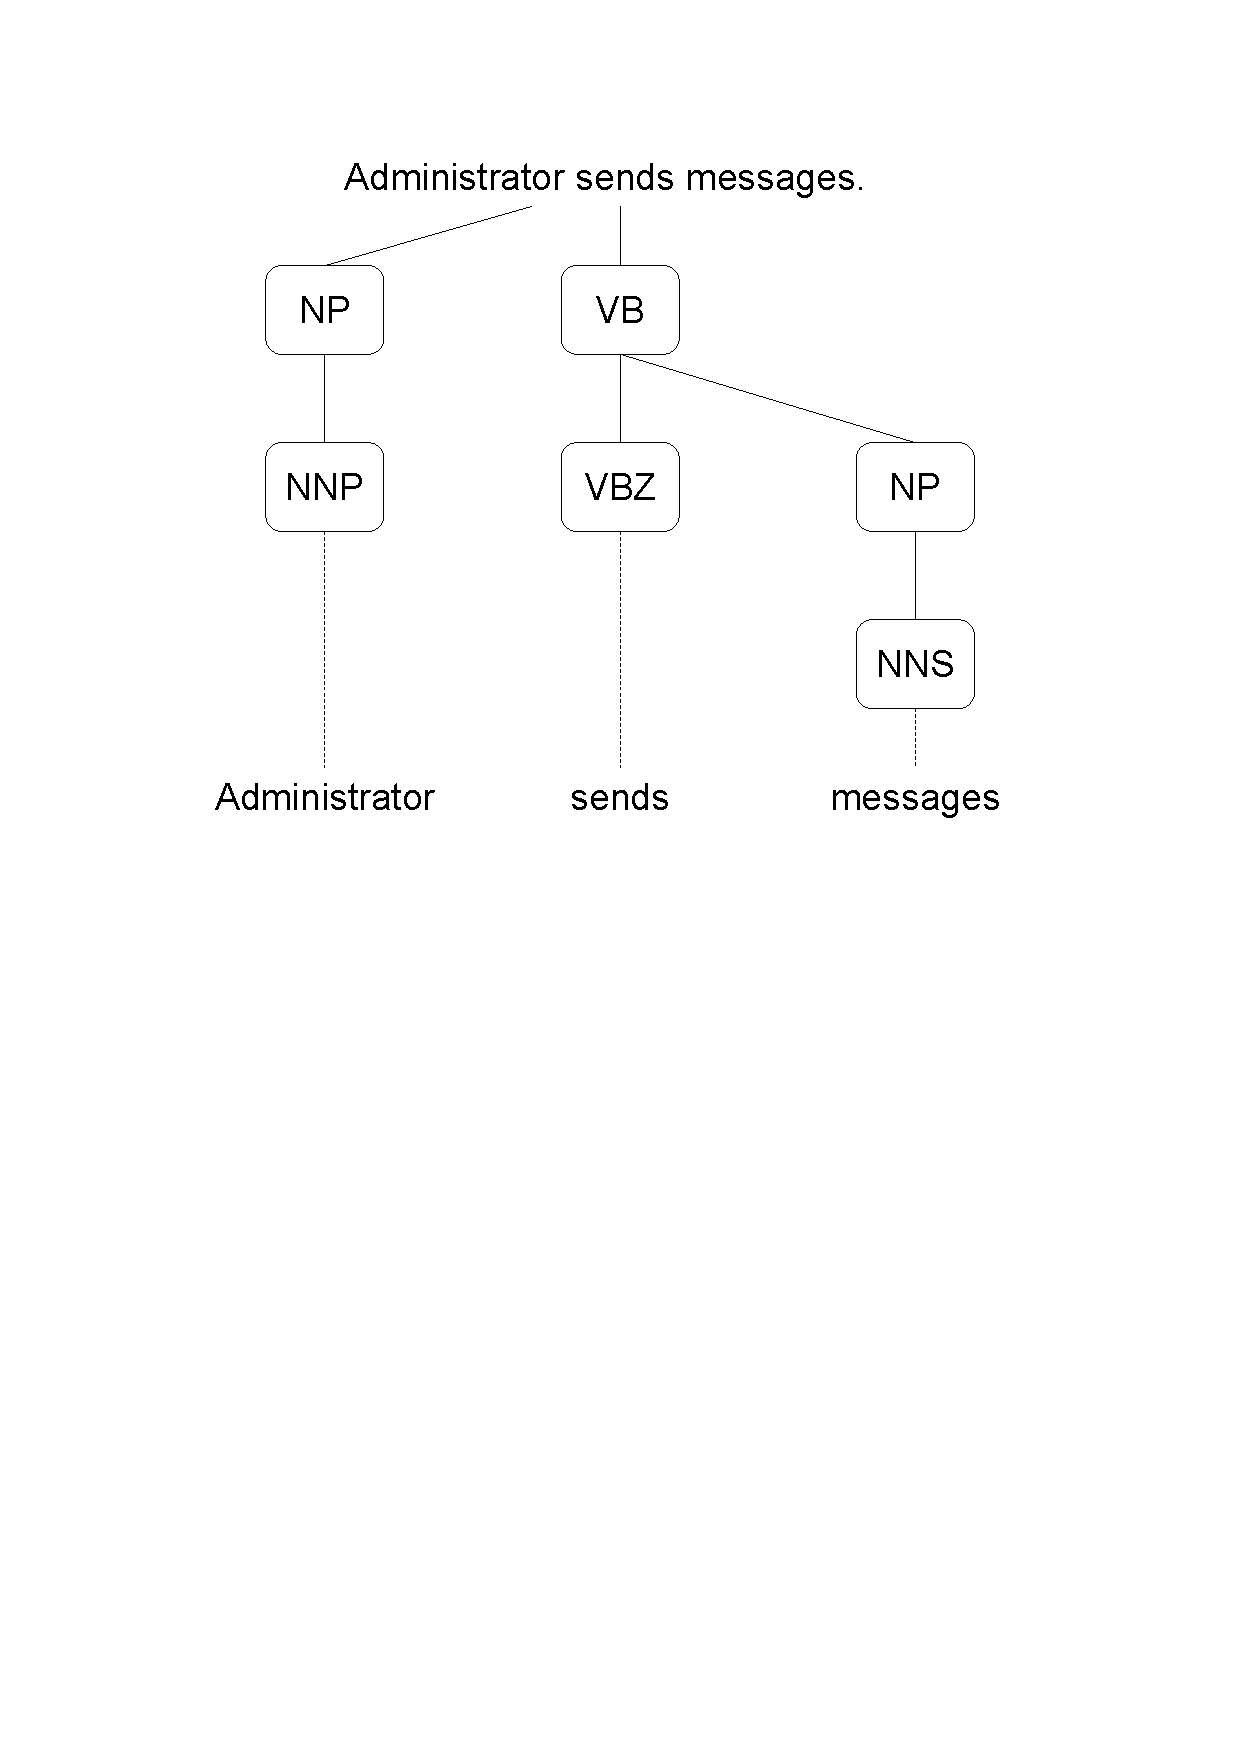
\includegraphics[width=200pt]{images/ParsedTree}
  \caption{Parsed tree of sentence "Administrator sends messages".}
  \label{fig:ParsedTree}
\end{figure}

\subsection{Analyzer}
\label{sec:analyzer}
This section contains two important parts. First is process of the whole linguistic analysis and the second is basic description of our core analyser.

\subsubsection{Analysis process}
This section contains description of set of all important analysis steps. We recommend to use this section as an entry point for reading \emph{Reprotool} source code.
Important linguistic model is shown at figure \ref{fig:ReprotoolLingModel}. 

First part of process is initialization. This process is executed at startup of \emph{Reprotool}:

\begin{itemize}
\item {\bf Initialize tagger} - external tagger is initialized.
\item {\bf Initialize parser} - external parser is initialized and started.
\item {\bf Initialize lemmatizer} - external lemmatizer is initialized started.
\item {\bf Analysis of the initialization sentence} - this step speeds up following analyses by memory initialization.
\end{itemize}

Initialization process is executed as Eclipse job and should take about ten seconds (depending on infrastructure). If initialization faces error, it tries to restart.\\

Second, bigger part on analysis process is sentence analysis. Its start is triggered by user pushing a button in IDE ( analyze command for use case step or in loop for all use case steps in use case). This process contains following steps:

\begin{itemize}
\item {\bf Execute linguistic analysis job for one sentence} - runs all four linguistic tools for selected sentence. When tools encounter error, analysis is executed with safe version of sentence with stripped bad characters. 
\item {\bf Match sentence object} - at this point we have original sentence string and sentence object with dependency tree. We have to match these objects for final action type text ranges marking.
\item {\bf Find text ranges} - analyze sentence for apostrophes and quotation marks. This step improves label targeting.
\item {\bf Execute core analyzer} - determines constituents and action types.
\item {\bf Prepare model changes} - stacks all needed changes of model. Changes must be valid and must corresponds.
\item {\bf Return results to UI} - all changes to model are executed at one place by UI. UI has always control over internal model.
\end{itemize}

When linguistic analysis are not able to analyze original sentence string, we create safe version of this string. This string contains only characters from set {\tt a-zA-Z0-9'".,?!:;}.

\subsubsection{Core analyzer}
Part of our project called "core analyzer" describes process following basic linguistic analysis. This core analyzer accomplish two main tasks:

\begin{itemize}
\item {\bf Determine constituents} - find all important words in sentence.
\item {\bf Determine action type} - set final action type.
\end{itemize}

Rules for determining constituents are described in own section \ref{sec:lingbackground}. Constituents are determined in order: subject, main verb, indirect object, representative object.

Also action types have own section \ref{sec:actiontypes}. These types are determined in order: Include, Goto, Abort, Internal, To system, From system. Rules for last three types are mostly used at same time.

All changes made by core analyzer are stored in \verb|CompoundCommand| object. Therefore, all changes are made at one place an user can undo these changes.

\begin{figure}[ht]
  \centering
  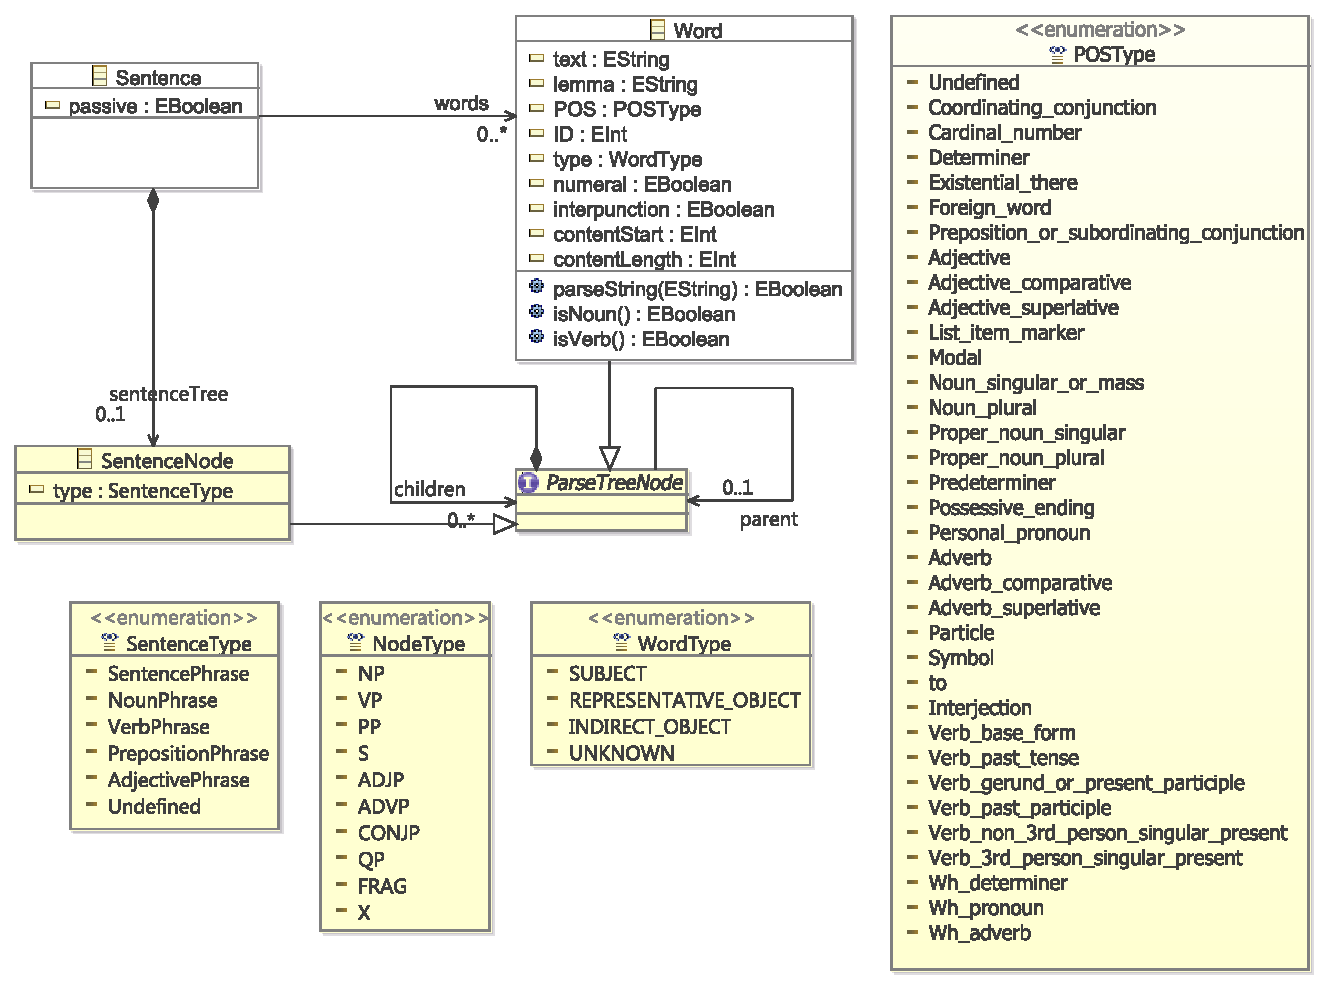
\includegraphics[width=\textwidth]{images/ReprotoolLingModel}
  \caption{Internal linguistics model with enumerations.  Model use Penn TreeBank tags notation.}
  \label{fig:ReprotoolLingModel}
\end{figure}

\subsection{Linguistics constituents background}
\label{sec:lingbackground}
Main goal of linguistic analysis in our project is to identify important words in a sentence. These words are mainly constituents. For our purpose, we are identifying four groups of words:

\begin{itemize}
\item {\bf Subject} main subject of the sentence
\item {\bf Main verb} verb which specifies meaning
\item {\bf Representative object} main subject of sentence action
\item {\bf Indirect object} an actor to whom or for whom the action of the verb is done and who is receiving the \emph{Representative object}
\end{itemize}

These words are used in action analysis. We are matching sentences to proper actions with a set of deriving rules, which are based on these words. 
                                                                    
\subsubsection{Subject}
For our purpose, subject must be always an actor. User has to add sentence actors before analysis. Usually is subject noun in a top noun phrase. If the sentence is in passive, subject stands at object's place. 

Subject could be also missing. In that case analysis still tries to find other constituents.

There are no predefined actors. Automatic analysis uses just project actors, but it is strongly recommended, that user adds "system" and "user" actors to project.

\subsubsection{Main verb}
This verb is a main verb of highest verb phrase in a sentence. In a passive sentence is auxiliary verb ignored. 

Finding verb in properly parsed sentence is an easy task, but in a sentence with a wrong parsed tree it usually can not be resolved. It happens usually when parser doesn't know contained verb. This means, that parser tags verb by different POS tag.

\subsubsection{Indirect object}
Indirect objects are derived before representative (conceptual) objects. All indirect objects are actors and indirect objects aren't in the same node with other objects.

Node with indirect objects must be a noun phrase containing verb phrase. If this node is found, all objects are marked as indirect. Indirect object cannot be in possessive form.  

\subsubsection{Representative object}
Representative object could be noun in a noun phrase which is a child of main verb phrase. Except noun phrase with indirect objects.

If a phrase contains more nouns without conjunction, we mark as an object last of the nouns. This rule was established, because external tools usually determine adverbs as nouns. After all, noun with multiple adverbs still represents one object.

\subsection{Action types deriving rules}
\label{sec:actiontypes}
When we have determined all constituents, analysis can continue with determining proper action type. This is followed by filling internal models with obtained data from analysis. Each action type has its own set of deriving rules and these rules are strictly disjunct. This means, that only one action type can be assigned to analyzed sentence. This section contains description of these deriving rules. 

There is only one important keyword, that our analysis use. It is "system" and determines analysis of To system and From system actions. 

When we talk about system, we talk about main base entity in project. This entity usually represents main part of application, or main decision making unit.

\subsubsection{Include use case action}
Sentence contains one of the following verbs: "continue", "repeat", "resume", "retry" and "include".  This verb must be main verb of the sentence. It also has to contain reference to usecase and label of one existing usecase in current project. For better determination of this action type is recommended to use word "usecase" in sentence.

\subsubsection{Goto action}
Sentence contains one of the verbs from \emph{Include use case action}. This verb must be main verb of the sentence. In addition, target of the action must be found and it has to be existing use case step in current use case. 

\subsubsection{Abort action}
Set of abort verbs contains "abort", "terminate", "end", "exit" and "finish".  This verb must be main verb of the sentence.

\subsubsection{From system action}
System is the subject of the sentence and we have identified indirect object (other than system). System is communicating with other actor.

\subsubsection{To system action}
System is an indirect object. Subject cannot be system. Example of \emph{To system} action could be found at figure \ref{fig:ToSystemActionExample}. In common use case, this action type represents communication from subsystems to system.

\subsubsection{Internal action}
System is a subject and there is no indirect object, or system is also indirect object. This action type is used for majority of common system actions, like sending messages or throwing errors.

\begin{figure}[ht]
  \centering
  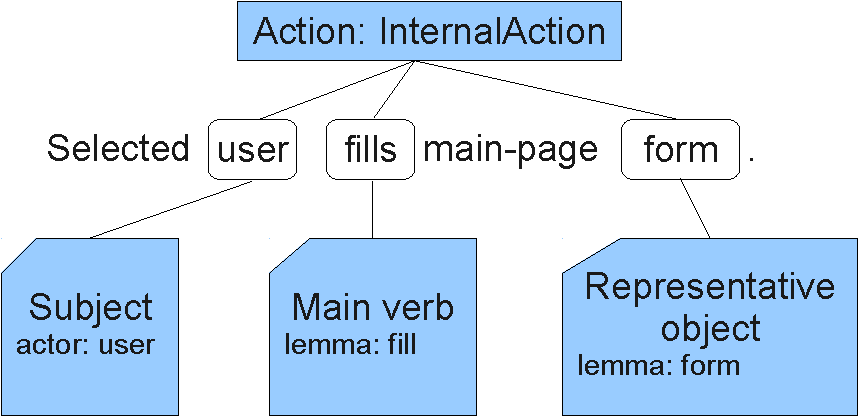
\includegraphics[width=250pt]{images/ToSystemActionExample}
  \caption{Example of To system action analysis result.}
  \label{fig:ToSystemActionExample}
\end{figure}

\subsubsection{Unknown action}
This is an default action type. If analysis could not find any other action, we set Unknown action type. This action type is also used when automatic analysis encountered error. 

\subsection{Benchmark}
\label{sec:benchmark}

We needed bigger set of proper sentences during the implementation of automatic linguistic analysis. These sentences were used for common testing purposes. Growing complexity of \emph{Reprotool} model demanded more and more testing sentences. Creation of own independent testing tool was just a logical step.

We have created special benchmark plug-in. This plug-in complement JUnit tests used during implementation and is part of {\tt reprotool.ling.tests} bundle. Core function of this plug-in is batch sentence analysis. Benchmark contains three main parts:

\begin{itemize}
\item {\bf Loading} - reading file containing annotated dataset.
\item {\bf Analysis} - batch analysis of all sentences in dataset.
\item {\bf Results output} - computing main results in usable format.
\end{itemize}

Our benchmark plug-in is ready to use. Usage of its features needs almost no source code modification. User only has to specify dataset file location. For quick run of this benchmark locate JUnit tests in {\tt reprotool.ling.tests} bundle and change noted dataset file location. Default location is set to file "data.csv" located in bundle.

Right usage of our benchmark plug-in is described in following list. This process is composed of more nontrivial tasks, but these tasks are easy to resolve.

\begin{enumerate}
\item {\bf Reprotool initialization} You have to be able successfully build our \emph{Reprotool} project. It is supposed, that user modifying our project is able to build Eclipse plug-in projects.
\item {\bf Obtaining sentences} First part of dataset creation is collecting data. It is recommended to obtain sentences from use cases.
\item {\bf Manual annotation} The most time consuming part is dataset annotation. Example of dataset file is located in table \ref{tab.benchmarkinput}.
\item {\bf Dataset location} User has to specify dataset location in source code.
\item {\bf Benchmark running} The easiest way to run benchmark is to execute corresponding JUnit test by right clicking on test file in Eclipse and selecting \emph{Run as} and \emph{JUnit Plug-in test}.
\end{enumerate}

Obtaining of proper dataset is more described in section \ref{sec:dataset}. 

\subsubsection{Implementation}
Benchmark plug-in uses same core functions like common \emph{Reprotool} linguistic analysis. Implementation of benchmark is slightly different from common analysis, because of data conversion an reading. We defined just two benchmark objects. First, main object, represents whole benchmark. Second object represents small version of one project. This small version of project comes from one dataset sentence. This means, that benchmark creates one project for each sentence. Main object contains list of these objects.

This difficult description could be better explained by following process. This process describes lifetime of one benchmark.

\begin{enumerate}
\item {\bf Main benchmark object is initialized} This step just sets up benchmark base properties,for example location of dataset.

\item {\bf Benchmark loads dataset} Benchmark locates dataset and in loop creates small project object for each sentence.
    \begin{enumerate}
    \item {\bf Loading sentence} Sentence with annotation is parsed. Representative results are created from annotation.
    \item {\bf Creating project} Benchmark creates project due to \emph{Reprotool} model. Benchmark sets up project, UseCase, Scenario, UseCaseStep and other needed objects.
    \item {\bf Linking objects} Benchmark links all objects, so the loaded sentence is not different from common UseCaseStep sentence.
    \end{enumerate}

\item {\bf Analyzing sentences} Benchmark analyzes each input sentence (now project)  like common project.
    \begin{enumerate}
    \item {\bf Linguistic tools} Parsed tree is created for each sentence.
    \item {\bf Action type} Analyzer tries to determine UseCaseStep action type.
    \item {\bf Store results} Important results are stored for each sentence.
    \end{enumerate}
\item {\bf Computing benchmark results} Benchmark computes final results from whole dataset. These results are printed to console. Example benchmark output is shown in table \ref{tab.benchmarkexample}.
\item {\bf Benchmark cleanup} Destruction of objects and termination.
\end{enumerate}

The most important part of benchmark are final results and their format. Result are computed for each annotated entity. Results for each entity consists of overall string. For example "{\tt OBJECTS: Count: 21 Found: 11 | 52,4\%}". This line is usually followed with set of lines containing errors. Each line starts with sentence identification, input (annotated) result and  output (analyzed) result. These informations are very important for localizing differences between input and output results.

Based on these informations, \emph{Reprotool} model can be changed for modified usage of our project to suit your needs.

\begin{table}[ht]   % or b
\begin{center}
    \begin{verbatim}
SUBJECTS: Count: 21 Found: 19 | 90,5%
RPT6: in-subjectNumber: 6 out-subjectNumber: 1
MOD1_UC1_7: in-subjectNumber: 0 out-esubjectNumber: 3
VERBS: Count: 21 Found: 20 | 95,2%
MOD1_UC1_5: in-verbLemma: "verify" out-verbLemma: "be"
INDIRECT_OBJECTS: Count: 21 Found: 20 | 95,2%
LING2: in-indirectObjectNumber: 8 out-indirectObjectNumber: 0
OBJECTS: Count: 21 Found: 11 | 52,4%
RPT8: in-objectNumber: 2 out-objectNumber: 0
LING1: in-objectNumber: 8 out-objectNumber: 4
MOD1_UC1_7: in-objectNumber: 3 out-objectNumber: 0
MOD1_UC1_8: in-objectNumber: 0 out-objectNumber: 5
TOTAL: Count: 84 Found: 70 | 83,3%   
    \end{verbatim}
  \caption{Example output from benchmark plugin}
  \label{tab.benchmarkexample}
\end{center}
\end{table}   
      
      
\subsubsection{Dataset}
\label{sec:dataset}
Most important precondition for benchmarking is good properly annotated dataset. In this section we would like to describe our annotation. It is recommended to see our annotated dataset before creation of other dataset.

We have defined eight basic sentence entities to annotate. These list could be followed with action type parameters. First entity is sentence identification string. This string is used for referencing to sentences, so it should be unique string for each sentence.

Entities are described in the following list:

\begin{enumerate}
\item {\bf ID } Id string for one sentence provided for sentence identification
\item {\bf SENTENCE } Test sentence
\item {\bf ACTORS } List of sentence actors (separated by commas)
\item {\bf SUBJECT\_NUMBER } Word index of subject
\item {\bf VERB\_LEMMA } Lemma form of main verb in a sentence
\item {\bf OBJECT\_NUMBER} List of objects indices
\item {\bf INDIRECT\_OBJECT\_NUMBER} Index of indirect objects (all indirect objects are in same sentence tree node)
\item {\bf ACTION\_CODE} Code of sentence action (sentence action type codes are described lower). 
\item {\bf ACTION\_PARAM1} First parameter of an action
\end{enumerate}   
   
There are few basic advices for annotation. All indices are starting from value 1. Value 0 indicates missing entity. Empty string in action code indicates Unknown action type. 

As mentioned in previous section, we have defined several action types. Each type should be also set in benchmark dataset. Defined action codes for corresponding action types are:      
     
\begin{itemize}
\item {\bf INTERNAL} Internal action
\item {\bf FROM\_SYSTEM} From system action
\item {\bf TO\_SYSTEM} To system action
\item {\bf GOTO} Continue action (parameter is an UseCaseStep)
\item {\bf ABORT} Abort use case action
\item {\bf INCLUDE} Include action (parameter is an UseCase)
\item {\bf UNKNOWN} Undefined action
\end{itemize}     

Table \ref{tab.benchmarkinput} contains few annotated sentences. You can see that annotation covers main results of common UseCaseStep analysis. And this is exactly the main purpose of our dataset annotation.
      
\begin{table}[ht]   % or b
\begin{center}
    \begin{scriptsize}  
    \begin{verbatim}      
ID;SENTENCE;ACTORS;SUBJECT_NUMBER;VERB_LEMMA;OBJECT_NUMBER;INDIRECT_OBJECT_NUMBER;ACTION_CODE;
_ ACTION_PARAM1;ACTION_PARAM2
RPT1;User opens window.;;1;open;3;;TO_SYSTEM;;
RPT2;System creates a new object.;;1;create;5;;INTERNAL;;
RPT3;User fills login.;;1;fill;3;;TO_SYSTEM;;
MOD1_UC1_5;System verifies if data is correct .;;1;verify;4;;INTERNAL;;
MOD1_UC1_6;System informs that account has been created .;;1;inform;4;;INTERNAL;;
MOD1_UC1_7;Some obligatory fields were not filled.;;0;be;3;;INTERNAL;;
MOD1_UC1_8;Systems highlights the missing fields .;;1;highlight;5;;INTERNAL;;
MOD1_UC1_9;Back to step 4 .;;0;;4;;GOTO;4;
    \end{verbatim}
    \end{scriptsize}
  \caption{Example input for benchmark plug-in}
  \label{tab.benchmarkinput}
\end{center}
\end{table}      
      
Main part of our benchmark dataset was obtained from \href{http://www2.put.poznan.pl/en}{Poznan University of Technology}, their \href{http://www.se.cs.put.poznan.pl/knowledge-base/software-projects-database/use-cases-database-ucdb/use-cases-database-ucdb}{Use Cases Database (UCDB)} and it coverts one project "\href{http://ucdb.cs.put.poznan.pl/benchmark/2.f.n/srs/index.html}{Admission System version 2.0F (quantitative)}".  

Whole dataset contains 269 manually annotated sentences. This dataset could be used for better use case verification, e.g. for benchmarking in any other project.   

\subsubsection{Results}
Our benchmark plug-in provides computed results after each execution. Obtaining results for other set of annotated sentences is very easy. There is no need to post-process benchmark results in any way.

Actual benchmark results of dataset analysis are shown in table \ref{tab.benchmarkresults}. shows current benchmark results. Total result is 88,10\%. This number means, that 11,90\% of tagged entities is not correctly recognized.

\begin{table}[ht]   % or b
\begin{center}
\begin{tabular}{l r r r}
 & Count & Found & Result \\
\hline
SUBJECTS: & 269 & 249 & 92,57\% \\
VERBS: & 269 & 244 & 90,71\% \\
INDIRECT OBJECTS:& 269 & 260 & 96,65\% \\   
OBJECTS: & 269 & 200 & 74,35\% \\
ACTIONS: & 269 & 232 & 86,25\% \\
\hline
TOTAL: & 1345 & 1185 & 88,10\% \\
\hline
\end{tabular}

  \caption{Final benchmark results}
  \label{tab.benchmarkresults}
\end{center}
\end{table}    
 
As you can see, our analysis returns result corresponding to manual annotation in 88,10\% of all cases. This number also means, that 11,90\% of tagged entities is not correctly recognized.

Results also show accuracy of selected analysis subtasks. We have to remind, that reference results were provided by our manual annotation. It is not too difficult to obtain own, more independent results. Annotators have to only follow instructions in previous section.


  \appendix
  \section{List of Reprotool plugins}
\label{sec:plugins}

\subsection{Core model + IDE}

\begin{verbatim}
reprotool.model
\end{verbatim}
EMF model for Reprotool project, annotations and linguistic analysis attached to use case step.

\begin{verbatim}
reprotool.model.edit
\end{verbatim}
Generated Reprotool project label providers and adapter factories

\begin{verbatim}
reprotool.model.edit.ext
\end{verbatim}
Customized Reprotool project label providers and adapter factories

\begin{verbatim}
reprotool.model.editor
\end{verbatim}
Generated Reprotool project editor.

\begin{verbatim}
reprotool.model.utils
\end{verbatim}
Utility classes for EMF model manipulation.

\begin{verbatim}
reprotool.ide
\end{verbatim}
Project, Use case and Counter example editor, Reprotool project wizard, Sentence analysis view

\begin{verbatim}
reprotool.lts
\end{verbatim}
LTS EMF model

\subsection{Formal analysis}

\begin{verbatim}
reprotool.fm.nusmv
\end{verbatim}
Conversion between Reprotool project model and XText NuSMV model, parser of the
NuSMV counter example.

\begin{verbatim}
reprotool.fm.nusmv.lang
\end{verbatim}
XText NuSMV grammar definition and all runtime components (parser, lexer, linker, validation, etc.)

\begin{verbatim}
reprotool.fm.nusmv.lang.ui
\end{verbatim}
XText based NuSMV editor and all the other work-bench related functionality.

\subsection{Linguistic analysis}

\begin{verbatim}
reprotool.ling
\end{verbatim}
EMF model used for linguistic tools, linguistic analysis toolchain.

\begin{verbatim}
reprotool.ling.tests
\end{verbatim}
Tests and Benchmark of the ling. tools.

\begin{verbatim}
reprotool.tools.anna
\end{verbatim}
Wrapper plugin generated for lemmatizer.

\begin{verbatim}
reprotool.tools.dbparser
\end{verbatim}
Plugin for dbparser.jar + configuration and model (data) for Daniel Bikel's parser.

\begin{verbatim}
reprotool.tools.mxpost
\end{verbatim}
Plugin for mxpost.jar + data for MX post tagger.


\subsection{Import and export}

\begin{verbatim}
reprotool.ide.txtuc
\end{verbatim}
XText grammar definition for Textual use case editor and all runtime components (parser, lexer, linker, validation, etc.)

\begin{verbatim}
reprotool.ide.txtuc.ui
\end{verbatim}
XText based Textual use case editor and all the other work-bench related functionality.

\begin{verbatim}
reprotool.tools.txtImport
\end{verbatim}
Conversion from Textual use case to Reprotool project + wizard

\begin{verbatim}
reprotool.uml.export
\end{verbatim}
Export from Reprotool project to UML2 EMF model.

\subsection{Supporting plugins}

\begin{verbatim}
reprotool.maven.aggregator
\end{verbatim}
Maven project referencing other plugins for automated build on Jenkins CI server.

\begin{verbatim}
reprotool.maven.parent
\end{verbatim}
Common dependencies for maven projects.

\begin{verbatim}
org.eclipselabs.reprotool.branding
\end{verbatim}
Contains configuration, splashscreen and icons to style RCP application

\begin{verbatim}
org.eclipselabs.reprotool.product-plugin-based
\end{verbatim}
RCP product configuration (list of bundled plugins), needed for PDE build.

\begin{verbatim}
reprotool.exampleProjects
\end{verbatim}
Projects used in "Reprotool example projects" wizard.
%  \section{5 Minutes Tutorial}
% TODO: this section is a stub - add screenshots and more text

\begin{itemize}
 \item Start Reprotool
 \item Create new Reprotool Project using the wizard
 \item Create UC1, UC2
 \item Create Scenarios
 \item Create steps
 \item Add \emph{use:x} annotation
 \item Convert SW Proj to SMV
 \item Run Verification
 \item View the counterexample
 \item Export UML
 \item Export LTS
\end{itemize}


\bibliographystyle{splncs03}
\bibliography{bibfile,bibfile-nusmv,bibfile-eclipse,bibfile-linguistics}

\end{document}
